%% HEADER
%%%%%%%%%%%%%%%%%%%%%%%%%%%%%%%%%%%%%%%%%%%%%%%%%%%%%%%%%%%%%
\newcommand{\hyperrefpdfauthor}{}
\newcommand{\hyperrefpdftitle}{}
\newcommand{\hyperrefpdfsubject}{}
\newcommand{\hyperrefpdfkeywords}{}
\newcommand{\hyperrefpdfborder}{0}
\documentclass{wissdoc-kw-eng}

% \usepackage[german, english]{babel}
% \selectlanguage{english}

\newcommand{\eg}[0]{e.g., }
\newcommand{\ie}[0]{i.e., }
\newcommand{\etal}[0]{et~al.}
\newcommand{\floatwidth}[0]{\columnwidth}
\newcommand{\subfloatwidth}[0]{0.48\columnwidth}
\newcommand{\comment}[1]{}
\definecolor{Orange}{rgb}{1,0.5,0}


\newcommand{\todo}[1]{\textsf{\textbf{\textcolor{Orange}{[[#1]]}}}}

\usepackage{tikz}
\usetikzlibrary{decorations.pathmorphing,calc,shapes,shapes.geometric,patterns,snakes,matrix,arrows,positioning}

\usepackage{dcolumn}
\newcolumntype{d}[1]{D{.}{.}{#1}}
\usepackage{siunitx}
\DeclareSIUnit\dBm{dBm}

\usepackage[printonlyused]{acronym}
\renewcommand{\bflabel}[1]{\normalfont{\normalsize{#1}}\hfill} % keine serifenlose schrift für acronym
\usepackage{subfigure}

\usepackage{float}
\floatstyle{ruled}
\newfloat{listing}{htbp}{lop}[chapter]
\floatname{listing}{Listing}

\usepackage[hang,center,nooneline]{caption}
\captionsetup[figure]{font={small,sf}}
\captionsetup[table]{font={small,sf}}
\captionsetup[listing]{font={small,sf}}
\usepackage{etoolbox}


%% Normales LaTeX oder pdfLaTeX? %%%%%%%%%%%%%%%%%%%%%%%%%%%%
%% ==> Das neue if-Kommando "\ifpdf" wird an einigen wenigen
%% ==> Stellen benötigt, um die Kompatibilität zwischen
%% ==> LaTeX und pdfLaTeX herzustellen.
%\newif\ifpdf
%\ifx\pdfoutput\undefined
%    \pdffalse              %%normales LaTeX wird ausgeführt
%\else
%    \pdfoutput=1
%    \pdftrue               %%pdfLaTeX wird ausgeführt
%\fi


%% Fonts für pdfLaTeX %%%%%%%%%%%%%%%%%%%%%%%%%%%%%%%%%%%%%%%
%% ==> Nur notwendig, falls keine cm-super-Fonts installiert
\ifpdf
	\usepackage{ae}       %%Benutzen Sie nur eines dieser Pakete:
	%\usepackage{zefonts}  %%je nachdem, welches Sie besitzen.
\else
	%%Normales LaTeX - keine speziellen Fontpackages notwendig
\fi


%% Deutsche Anpassungen %%%%%%%%%%%%%%%%%%%%%%%%%%%%%%%%%%%%%
%\usepackage[T1]{fontenc}
%\usepackage[utf8]{inputenc}

%% zur Zitaten des Quelltextes%%%%%%%%%%%%%%%%%%%%%%%%%%%%%%%
% "final" forces printing of all listings, even if the global "draft" is set
\usepackage[final]{listings}
\lstset{
    basicstyle=\footnotesize\ttfamily,
    tabsize=4,
    numberstyle=\tiny\color{gray},
    numbersep=5pt,
    numbers=left,
    captionpos=b,
    abovecaptionskip=0pt,
    belowcaptionskip=0pt,
    aboveskip=10pt,
    belowskip=0pt,
    floatplacement=tbp,
    frame=topline,
    framerule=.1pt,
    framesep = 3pt,
    }
\renewcommand\lstlistingname{\textbf{Listing}}
% This is only kept for backwards compatibility. You should never have to use it. Use the listing-environment instead.
%\DeclareCaptionFormat*{lstruled}{{\bfseries#1\small\space\normalfont#3\hrule height.1pt depth0pt}\par}
%\captionsetup[lstlisting]{format=lstruled,singlelinecheck=false}

%% mehrere Abbildungen in eine %%%%%%%%%%%%%%%%%%%%%%%%%%%%%%
\usepackage{subfigure}

%% Packages für Formeln %%%%%%%%%%%%%%%%%%%%%%%%%%%%%%%%%%%%%
\usepackage{amsmath}
\usepackage{amsthm}
\usepackage{amsfonts}

%% Zeilenabstand %%%%%%%%%%%%%%%%%%%%%%%%%%%%%%%%%%%%%%%%%%%%
\usepackage{setspace}
%\singlespacing        %% 1-zeilig (Standard)
%\onehalfspacing       %% 1,5-zeilig
%\doublespacing        %% 2-zeilig


%% Andere Packages %%%%%%%%%%%%%%%%%%%%%%%%%%%%%%%%%%%%%%%%%%
%\usepackage{a4wide} %%Kleinere Seitenränder = mehr Text pro Zeile.
\usepackage{fancyhdr} %%Fancy Kopf- und Fußzeilen
%\usepackage{longtable} %%Für Tabellen, die eine Seite überschreiten
\usepackage{lscape}
\usepackage{rotating} 
%\usepackage[htt]{hyphenat} %Trennung von Typewriter-Schriften
%\usepackage{listings}
\usepackage{pstricks-add}
\usepackage[official]{eurosym}


% Tabellen mit Center und left
\usepackage{tabularx,colortbl} % colored table background
\newcolumntype{C}[1]{>{\centering\arraybackslash}p{#1}}
\newcolumntype{R}[1]{>{\raggedleft\arraybackslash}p{#1}}
% Table spacings
\newcommand\T{\rule{0pt}{2.5ex}\rule[-1.0ex]{0pt}{0pt}}
\newcommand\B{\rule[-1.0ex]{0pt}{0pt}}

\colorlet{slightgray}{black!20}
\colorlet{slightred}{red!30}
\colorlet{slightgreen}{green!30}
\colorlet{slightblue}{blue!30}
\colorlet{moteblue}{blue!60!black!20}
\colorlet{motered}{red!60!black!20}

%% Definitionen %%%%%%%%%%%%%%%%%%%%%%%%%%%%


%% zur Benutzung bei ergänzenden Daten%%%%%%%%%%%%%%%%%%%%%%%%
%\usepackage{endnotes}
%\renewcommand{\notesname}{Konfigurationsdaten der Messreihen}
%\renewcommand{\theendnote}{\Alph{endnote}}
%\renewcommand{\enotesize}{\normalsize}

%\hyphenation{Sensor-netz-werk
%}

%%%%%%%%%%%%%%%%%%%%%%%%%%%%%%%%%%%%%%%%%%%%%%%%%%%%%%%%%%%%%
%% DOKUMENT
%%%%%%%%%%%%%%%%%%%%%%%%%%%%%%%%%%%%%%%%%%%%%%%%%%%%%%%%%%%%%
\begin{document}

%% Dateiendungen für Grafiken %%%%%%%%%%%%%%%%%%%%%%%%%%%%%%%
%% ==> Sie können hiermit die Dateiendung einer Grafik weglassen.
%% ==> Aus "\includegraphics{titel.eps}" wird "\includegraphics{titel}".
%% ==> Wenn Sie nunmehr 2 inhaltsgleiche Grafiken "titel.eps" und
%% ==> "titel.pdf" erstellen, wird jeweils nur die Grafik eingebunden,
%% ==> die von ihrem Compiler verarbeitet werden kann.
%% ==> pdfLaTeX benutzt "titel.pdf". LaTeX benutzt "titel.eps".
%\ifpdf
%    \DeclareGraphicsExtensions{.pdf,.jpg,.png}
%\else
%    \DeclareGraphicsExtensions{.eps}
%\fi

\pagestyle{empty} %%Keine Kopf-/Fusszeilen auf den ersten Seiten.

\ifnotdraft{
%% Deckblatt %%%%%%%%%%%%%%%%%%%%%%%%%%%%%%%%%%%%%%%%%%%%%%%%
\frontmatter
\titlehead{
	\centering
	
\includegraphics[height=20mm,keepaspectratio]{thesis-tex/logos/comsys-text}
	\hfill
	
\includegraphics[height=20mm,keepaspectratio]{thesis-tex/logos/rwth}
} % end titlehead

\begin{titlepage}

\let\footnotesize\small \let\footnoterule\relax

\hbox{}
\vfill

\centering

\begin{doublespace} 
{ \huge\textbf{\textsf{Temperature Dependency \\ \vspace{-0.4em}
of Bit Error Distributions \\ \vspace{-0.4em}
in Wireless Sensor Networks \\ \vspace{-0.4em}}}}
\end{doublespace}
\vskip 2cm

{\large Bachelor Thesis\\[5pt]}
{\large \textbf{Niklas Hauser}}
\vskip 1cm

\textbf{RWTH Aachen University, Germany\\[5pt]
        Chair of Communication and Distributed Systems}
\vskip 2cm

\large

Advisors:
\vskip 2mm

\begin{tabular}{R{7cm}p{7cm}}
Dr. & Matteo Ceriotti\\
Dipl.-Inform. & Florian Schmidt\\
Prof.~Dr.-Ing. & Klaus Wehrle\\
Prof.~Dr.~rer.~nat. & Bernhard Rumpe
\end{tabular}
\vskip 1cm

\begin{tabular}{R{6cm}p{6cm}}
Registration date:  & January 29, 2014 \\
Submission date:    & May 29, 2014 \\
\end{tabular}

\vfill

\end{titlepage}


\cleardoublepage
\thispagestyle{empty}
\vspace*{36\baselineskip}
\hbox to \textwidth{\hrulefill}

I hereby affirm that I composed this work independently and used no other than the specified sources and tools and that I marked all quotes as such.

Hiermit versichere ich, dass ich die Arbeit selbstständig verfasst und keine anderen als die angegebenen Quellen und Hilfsmittel benutzt sowie Zitate kenntlich gemacht habe.

Aachen, den 29. Mai 2014

\cleardoublepage
\cleardoublepage

% \selectlanguage{german}

\begin{center}
\paragraph{Kurzfassung}
\hrulefill

\end{center}

Mit der Verfügbarkeit von leistungsfähigen eingebetteten Geräten und kostengün\-stigen Funkmodulen, beginnen auch immer mehr batteriebetriebene Sensorgeräte miteinander zu reden und Probleme gemeinsam zu entscheiden.
Es ist abzusehen, dass die Benutzung solcher intelligenten Geräte in drahtlosen Sensornetzwerken in\-dustrielle Prozesse vereinfachen und unsere Lebensqualität verbessern wird.

Allerdings ist die Laufzeit dieser mobilen Geräte durch ihre endliche Energiequelle, die meist nur mit viel Aufwand zu wechseln ist, beschränkt. Daher braucht es eine Programmierung, die energiebewusst kommuniziert, um die Lebensdauer der Bat\-terie so weit wie möglich zu verlängern.
Drahtlose Kommunikation ist stark durch Umweltveränderungen, allen voran die Lufttemperatur, beinflussbar, was zu Korrup\-tion oder Verlust von Paketen führen kann und ein erneutes Versenden des Pakets nach sich zieht.

In dieser Arbeit beschreiben wir eine kostengünstige Testplatform zum Testen der Funkverbindungen in einer temperaturkontrollierten Umgebung. Mit dieser Plat\-form untersuchen wir die Empfangsraten und die Bitfehlerverteilungen in korrupten Paketen.
Unsere Ergebnisse widerlegen frühere veröffentlichte Ergebnisse.
Schließ\-lich wenden wir diese Erkenntnisse auf die Programmierung eines Simulators an, mit dem wir untersuchen, wie sich Temperatur als Eingabegröße einer adaptiven Vorwärtsfehlerkorrektur verhält, um damit die Empfangsraten korrupter Pakete zu verringern.

% \selectlanguage{english}

\vspace {0.5cm}
\begin{center}
\paragraph{Abstract}
\hrulefill
\end{center}

With the availability of powerful embedded devices and inexpensive radio communication, ever more battery powered sensor devices make use of the added connectivity to talk to each other and decide problems collectively.
It is envisioned that usage of such smart devices in \acl{WSN}s will streamline industrial processes as well as improve our quality of life.

However, the runtime of these mobile devices is limited by their finite power source, which most often are impractical to exchange.
Therefore energy-aware programming and communication is required to prolong battery life for as long as possible.
Unfortunately, wireless communication is strongly influenced by environmental changes, most prominently air temperature, which can lead to packet corruption or loss and requires energy-consuming retransmissions.

In this work we describe a low-cost testbed for testing radio performance in a temperature-controlled environment, with which we examine packet reception rates and bit error distributions within packet corruption. Our results disprove previous published findings.
Finally, we apply these findings on building a simulator, with which we investigate using temperature as an input for an adaptive \acl{FEC} scheme to improve packet reception rates and thereby reduce unnecessary retransmissions.

\cleardoublepage
\cleardoublepage

\chapter*{Acknowledgments}



\cleardoublepage

% Titelseite hatte noch normale Tabellen. Von hier ab sollen alle
% Tabellen laut style-Vorgaben sans serif sein.
\AtBeginEnvironment{tabular}{\sffamily}
\AtBeginEnvironment{tabularx}{\sffamily}

%% Inhaltsverzeichnis %%%%%%%%%%%%%%%%%%%%%%%%%%%%%%%%%%%%%%%
\tableofcontents %Inhaltsverzeichnis
\cleardoublepage %Das erste Kapitel soll auf einer ungeraden Seite beginnen.
} % end ifnotdraft

\pagestyle{fancy} %%Ab hier die Kopf-/Fusszeilen: headings / fancy / ...

%%%%%%%%%%%%%%%%%%%%%%%%%%%%%%%%%%%%%%%%%%%%%%%%%%%%%%%%%%%%%
% einzelne Kapitel
%%%%%%%%%%%%%%%%%%%%%%%%%%%%%%%%%%%%%%%%%%%%%%%%%%%%%%%%%%%%%
%\include{commands}

\mainmatter
\chapter{Introduction}



\chapter{Background}


\chapter{Related Work}
\label{chap:related_work}

The research field of investigating influences of the environment on wireless link quality is large and spans many technologies and protocols.
However, we focus on technologies deployed in low power networks such as \ac{WSN}s, where the advances in small and affordable radio technology pushed research forward.
In a first step towards energy efficient, reliable communications, especially in battery powered applications, a deep understanding of why messages become corrupted is required.

Here we present research relating to the IEEE 802.15.4 protocol used in most \ac{WSN}s, especially in the three areas this work focuses on, namely, the influence of temperature on link quality and bit error distributions within corrupted messages, as well as the use of \ac{FEC} to counteract these effects.


\section{Effects of Temperature}

Bannister~\etal~\cite{Bannister2008} were one of the first to systematically investigate the effect of temperature on the performance of the CC2420 radio.
They connected two radios together via coaxial cable with attenuators and placed one of them in a thermal chamber with a temperature range of 25 to \SI{65}{\celsius} while measuring signal power using the \ac{RSSI}.
The results showed a reduction of output power by $4--$\SI{5}{\dBm} when the transmitter was heated, but only \SI{3}{\dBm} reduction in measured input power when the receiver was heated.
Boano~\etal~\cite{Boano2010} also investigated this behavior in 2010 in a real world deployment, but found no difference in \ac{RSSI} between transmitter and receiver.
However, both works point to a loss of gain in the CC2420 \ac{LNA} as the source of the reduction in signal powers at higher temperatures.

In a long-term outdoor study in 2013, Wennerstr{\"o}m~\etal~\cite{Wennerstrom2013} examined the correlation between \ac{RSSI} and \ac{PRR} and environmental factors, such as temperature, relative and absolute humidity, precipitation and sunlight.
They found that of all environmental factors, temperature had the strongest influence, with an increase in temperature causing a significant decrease in both \ac{RSSI} and \ac{PRR}.
This was further researched by Boano~\etal~\cite{Boano2013}, who focused on the impact of temperature on \ac{RSSI}, \ac{SNR}, Noise Floor, \ac{PRR} and \ac{LQI}.
They determined a negative impact of temperature on all these values and expanded their work by looking at the asymmetry of \ac{PRR} when heating the transmitter and receiver.
They found that the loss in \ac{PRR} was more pronounced when heating the transmitter than the receiver.

Finally, Z\'{u}\~{n}iga~\etal~\cite{Zuniga2013} created a summarizing report on the effect of environment variables on current \ac{WSN} motes.
Apart from including all previous findings, they also describe a substantial negative impact of temperature on microcontroller clock drift.
However, the CC2420 clock is compensated for temperature and experiences no such drift.


\section{Bit Error Distributions}

Liang~\etal~\cite{Liang2010} investigated bit error distributions in the context of 802.11 (WiFi) interference.
They found that packet collisions cause burst errors, due to 802.11 packets typically being much shorter than 802.15.4 packets, particularly in the beginning of a message.
This is due to the 802.11 sender deferring sending its packets until the 802.15.4 transmission completed, however only if the 802.15.4 sender is close enough so that its transmission power can be sensed by the 802.11 collision avoidance algorithm.
If the 802.11 sender cannot sense the 802.15.4 transmission, the authors show an even bit error distribution across the entire packet.

Schmidt~\etal~\cite{Schmidt2013} examined the bit error distributions within corrupted messages in their outdoor testbed of 20 TelosB devices.
Similar to Liang~\etal, they found that for random payload, \ac{BER} remains stable throughout message, however, within all 4-bit symbols, the \ac{MSB} is significantly less likely to break than the 3 \ac{LSB}.
In addition, symbols with \ac{MSB} set to 1 are more likely to break than symbols with \ac{MSB} set to 0.
This behavior creates very different Hamming distances between the broken symbols coded in 32-bit chip sequences than defined by the 802.15.4 standard.
The authors also looked at burst error distribution and found these errors not independently distributed, but skewed towards longer bursts.

Their findings then where further completed by Hermans~\etal~\cite{Hermans2014} with an understanding of why the Hamming distances are different than expected.
The authors discovered that the pattern fits, when their simulation of these patterns uses a \ac{MSK} instead of the \ac{OQPSK} demodulator suggested by the 802.15.4 standard.
The \ac{MSK} demodulator can correctly receive packets sent by an \ac{OQPSK} modulator, but it outputs different code words than defined by the standard.
The authors hypothesized that these code words then have to be translated using a table, which would create the distinct bit error patterns.


\section{\acl{FEC}}

The use of \ac{FEC} schemes in communication has been investigated before, however, the available limited resources on \ac{WSN} motes focus research in this area very much on coding and energy efficiency.

Jeong~\etal~\cite{Jeong2003} investigated the performance of single- and double-bit correcting \ac{ECC} on very early \ac{WSN} motes, not using the 802.15.4 standard.
They came to the conclusion, that using \ac{BCH} codes is simple to implement, but performs poorly when encountering burst errors.
Busse~\etal~\cite{Busse2006} then compared the performance of a Hamming code, an interleaved double-bit correction code and a \ac{RS} code using their \ac{WSN} and found the \ac{RS} code to be the most efficient of them, both in the length of the added overhead, as well as the error correction capabilities.

Using mathematical energy consumption modeling, Tian~\etal~\cite{Tian2008} showed that for small packet lengths ($<1023$ bytes) \ac{BCH} codes outperform \ac{ARQ}.
However, research by Ma~\etal~\cite{Ma2009} points to \ac{RS} being more energy efficient than \ac{BCH} codes, especially when considering the energy consumption of transmitting the coding overhead.

Ahn~\etal~\cite{Ahn2005} examined changing \ac{FEC} coding strength dynamically based on link quality properties.
Their adaptive \ac{FEC} algorithm outperformed several static \ac{RS} codes in simulation, as well as in real traces.
Liang~\etal~\cite{Liang2010} created and evaluated an efficient, TinyOS compatible \ac{RS} implementation, called TinyRS, during their research on bit error distributions mentioned before.







\chapter{Testbed Description}
\label{chap:testbed}

In order to be able to investigate the effects of temperature on our \ac{WSN} motes, we built a new low-cost testbed, which can accurately control mote temperature and allows the mote to maintain a certain antenna position.
Furthermore, we wrote flexible control and evaluation software, which orchestrates the experiments and logs all relevant data to disk.
In this chapter we will describe the design decisions we made and how they influence the testbed performance.

\section{Temperature Box}
\label{sec:temperature_box}

For our experiments we needed a way to accurately control temperature of motes in our \ac{WSN}.
Even though previous setups used an infrared lamp~\cite{Boano2014, Hermans2013} to heat the motes directly, we chose to control mote temperature only using air temperature.
The mote is placed in a closed \ac{PS} hard-foam box and the confined air is heated to the requested temperature and circulated to transfer this heat to the mote.
The box has the outside dimensions of \SI{35 x 35 x 30}{\centi\metre} with a wall thickness of \SI{5}{\centi\metre} which results in a holding capacity of \SI{12.5}{\litre}.

\subsection{Hardware}
A microcontroller evaluates temperature sensors within the box and locally controls the duty cycles of a small fan and a \SI{150}{\watt} ceramic heating element using a closed-loop \acs{PID} controller to achieve the requested air temperature.
The microcontroller can communicate over a serial connection to receive the desired temperature and send the current temperature.

Additionally, air temperature is displayed as a hue from blue (cold) via green (warm) to red (hot) on a RGB LED.
The duty cycles of the heating element and fan are mapped to two white LEDs, to provide an immediate status overview and prevent burn injuries.

The box is powered by a \SI{300}{\watt} PC power supply, which was chosen for its ability to provide \SI{12}{\volt}, \SI{5}{\volt} and \SI{3.3}{\volt} at the required currents, which removes the need for additional (costly) voltage conversion.
A custom designed PCB distributes power from the \acs{ATX} connectors to two high and two medium power \acs{MOSFET} switches and up to five temperature sensors, all controlled by an ATmega328.

The PCB, heating element and fan are fixed on a wooden baseplate shown in Figure~\ref{fig:box_hardware_picture} using custom fasteners and standard screws.
All custom made parts were prototyped using the PCB mill and laser cutter of the RWTH FabLab~\cite{fablab}.

\begin{figure}[t]
	\centering
    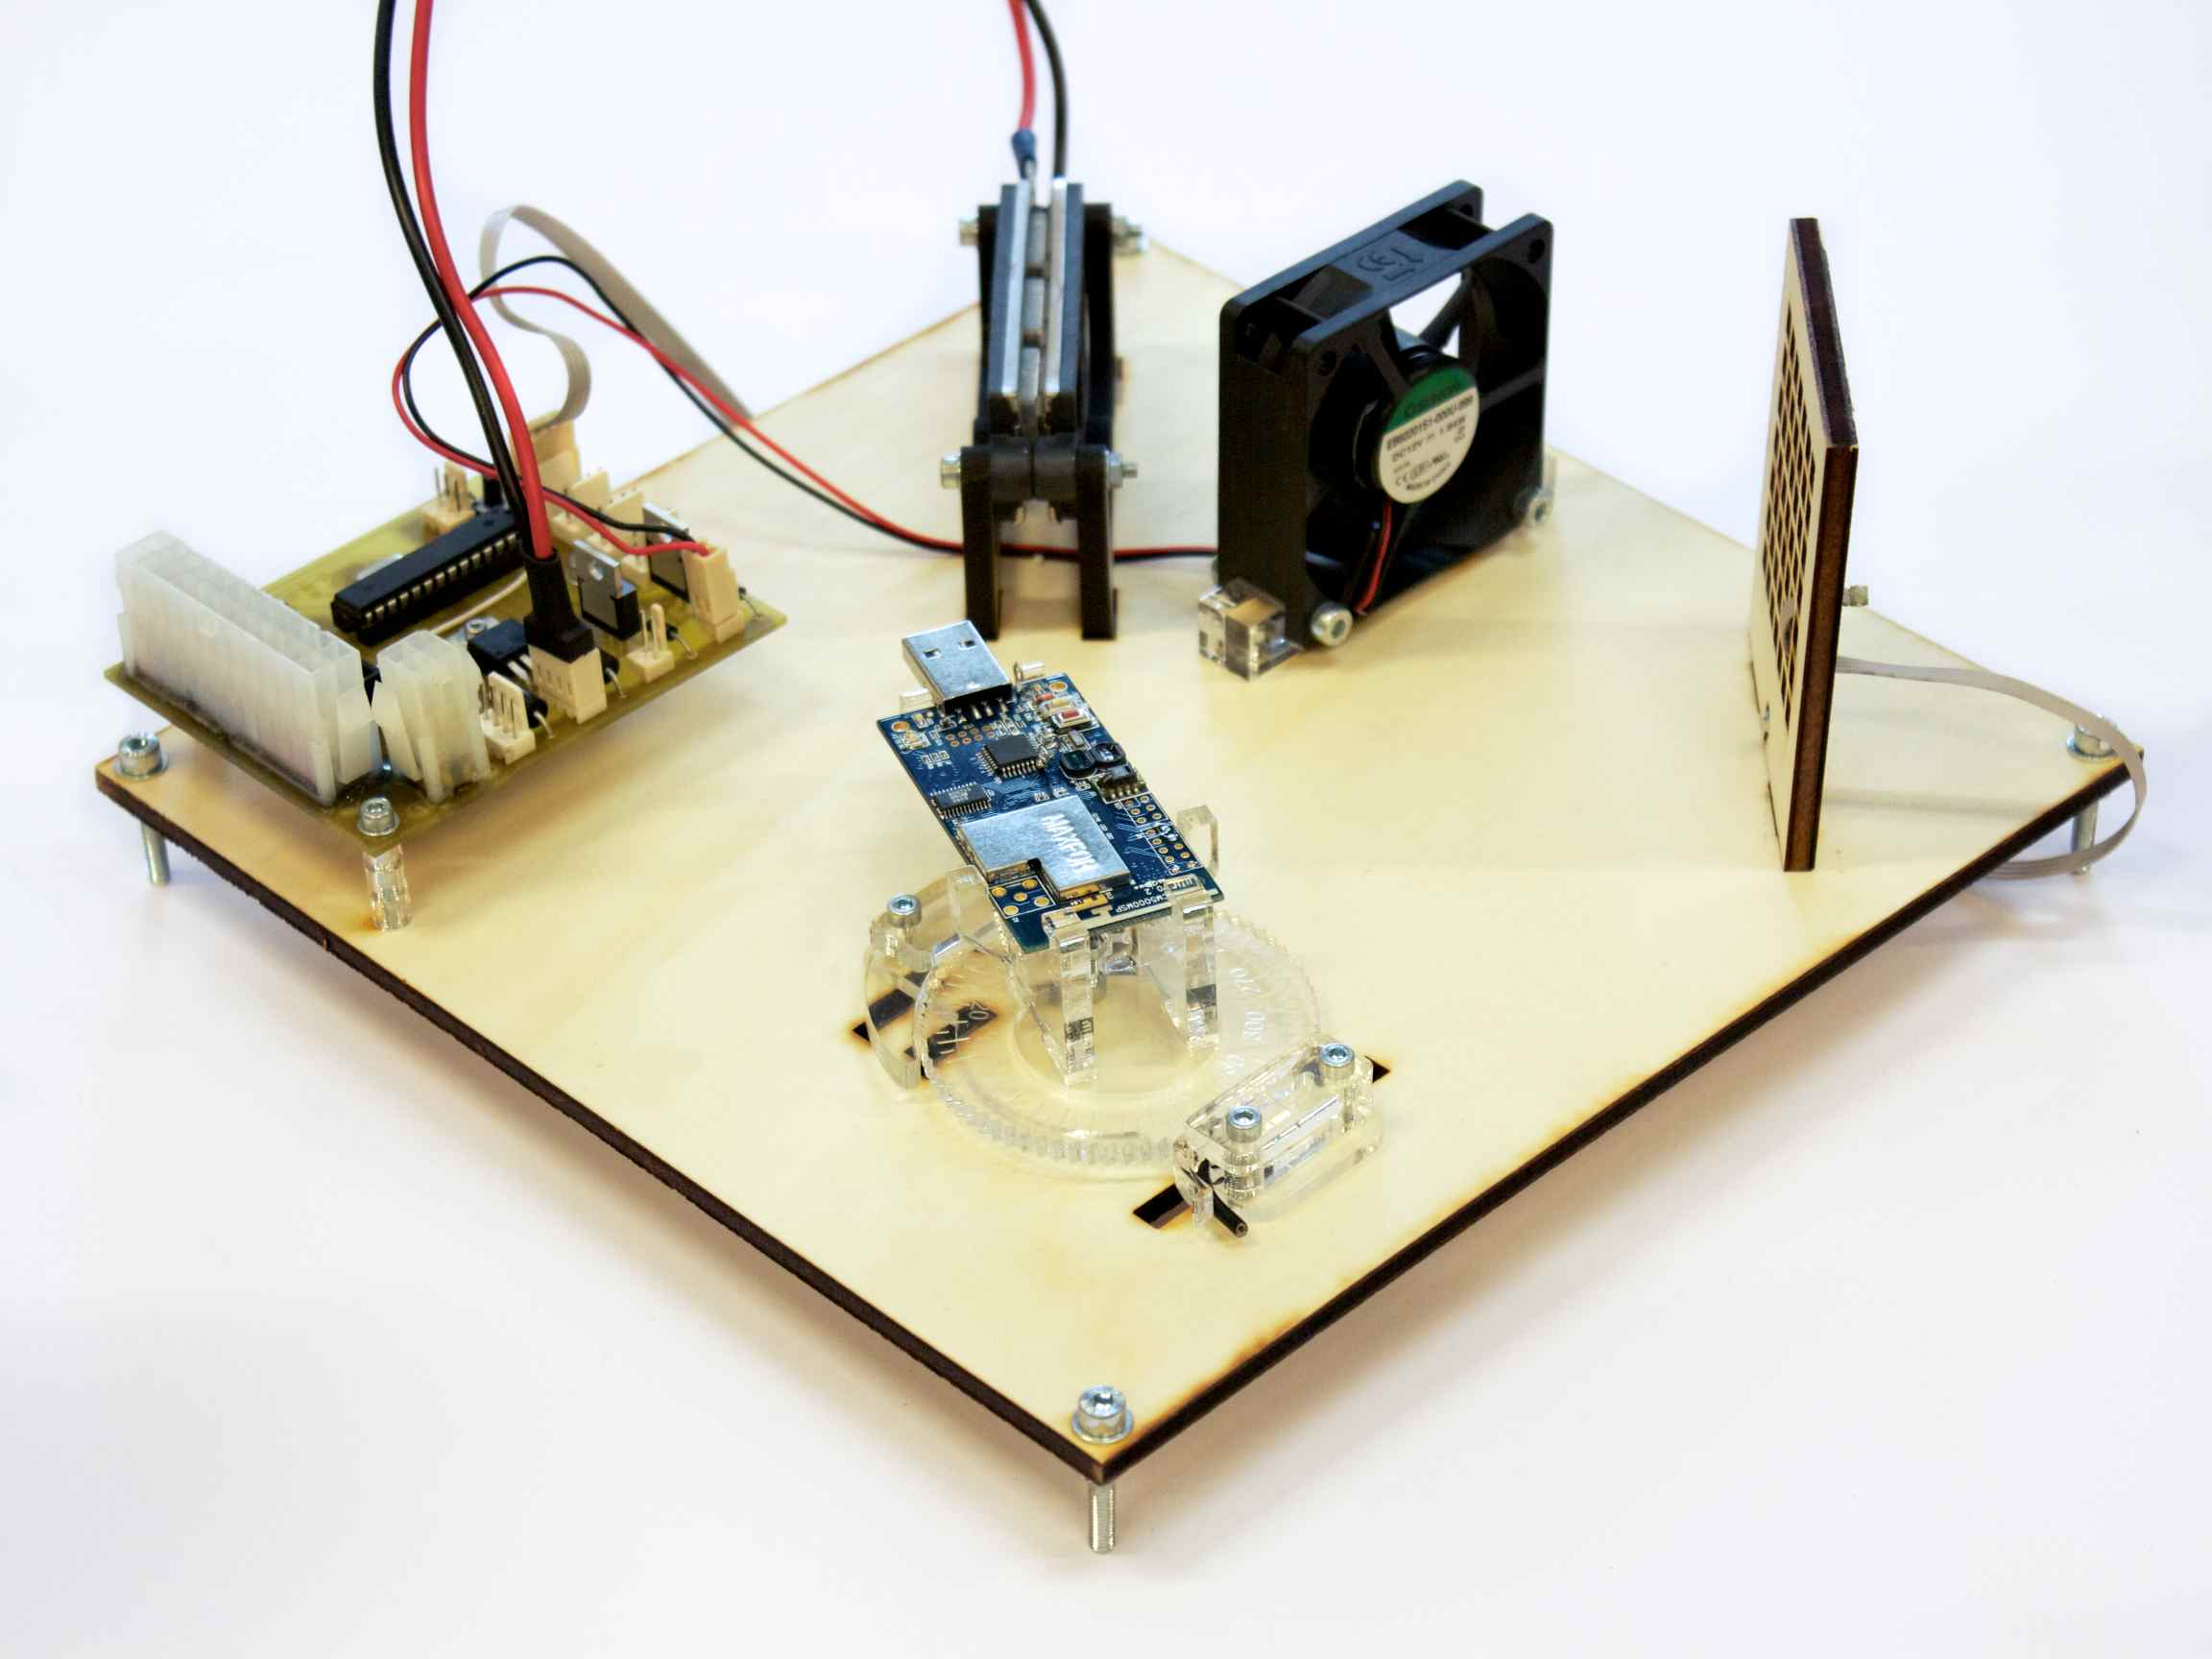
\includegraphics[width=1\columnwidth]{figures/temperature_box}
	\caption{Baseplate with temperature controller, heating element, fan and sensor mote.}
    \label{fig:box_hardware_picture}
\end{figure}


\subsection{Embedded Software}

The embedded software is written in C++ using the xpcc microcontroller framework~\cite{xpcc.io} and implemented as a set of asynchronous control tasks for input parsing and output formatting, temperature sensor evaluation, \acs{PID} loop update and duty cycle generation.
The choice of an ATmega328 as a microcontroller was deliberate to enable compatibility with the Arduino framework, which might be more familiar to developers.

Once the controller is programmed via \ac{ISP}, it will periodically send the values of all attached temperature sensors, as well as the current heating element power setting in human-readable ASCII format.
Desired temperature can be sent as an ASCII formatted integer followed by the letter `C'.
All switching frequencies were kept well below \SI{1}{\kilo\hertz} to avoid any kind of interference with the \SI{2.4}{\giga\hertz} band.


\subsection{Performance}

The heating element has enough power to heat the air inside the box up to \SI{120}{\celsius}.
This can however damage both the \ac{PS} material as well as the mote, so a hard limit of \SI{90}{\celsius} is imposed during experiments.

As seen in Figure~\ref{fig:box_heating_cooling} it takes about 40 minutes to heat up to \SI{90}{\celsius} and about 2 hours to cool back down to \SI{30}{\celsius}.
The \acs{PID} loop is deliberately dampened so that no overshoot in air temperature occurs, however, since the mote temperature naturally lags behind, a slight overshoot in air temperature might actually help achieve desired mote temperature quicker.
However, during the experiments a more granular approach is used similar to Figure~\ref{fig:box_heating_step}.

The boxes can be retrofitted with an active piezoelectric cooling element and a fan by connecting them to the two unused \acs{MOSFET} switches on the controller and updating the software, which also allow reaching temperatures below room temperature.
Since we did not use a cooling element, we set the minimum experiment temperature at \SI{30}{\celsius} so that in a room temperature of $20-$\SI{25}{\celsius} it can still be reached within reasonable time.

\begin{figure}[t]
	\subfigure[Heating to \SI{90}{\celsius}, then cooling to \SI{30}{\celsius}.] {
    	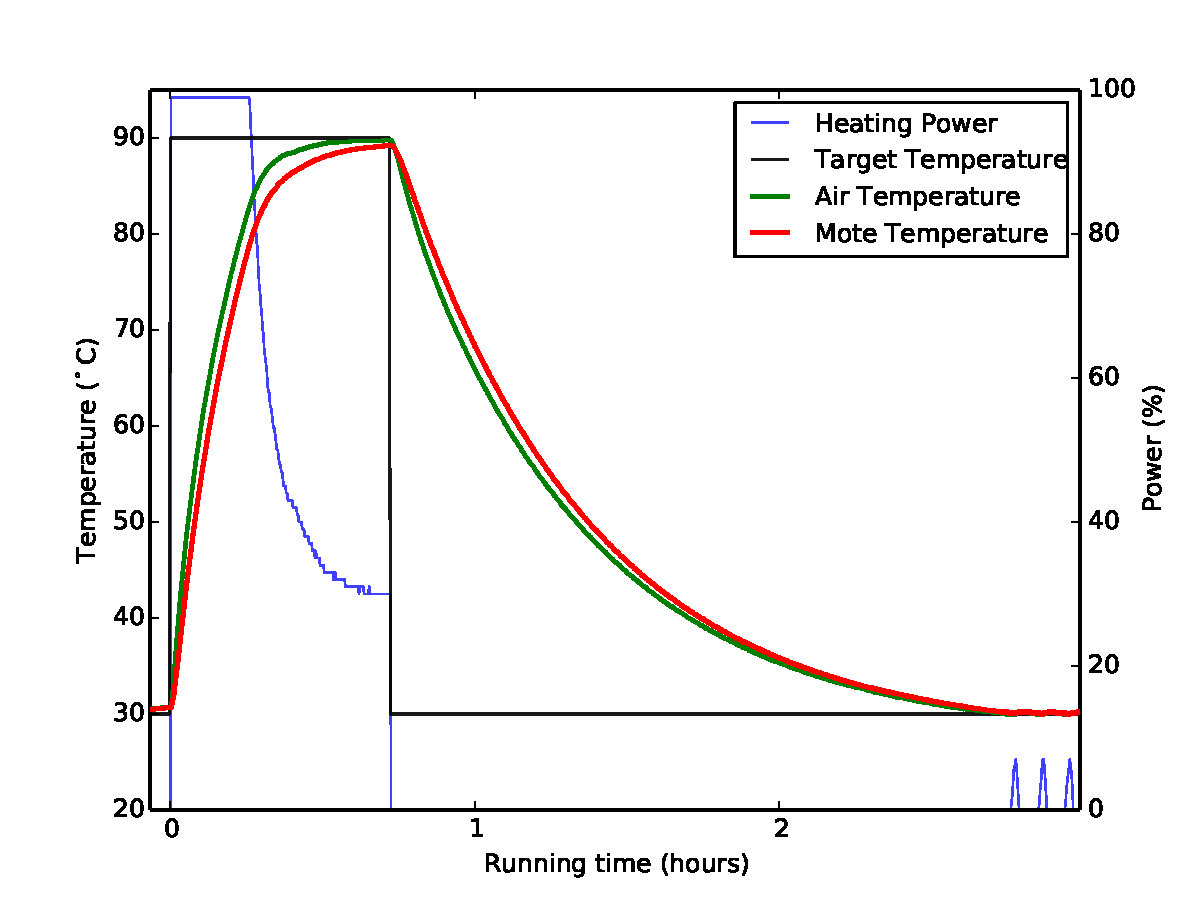
\includegraphics[width=0.475\columnwidth]{figures/box_heating_cooling}
    	\label{fig:box_heating_cooling}
    }
    \subfigure[Temperature increments of \SI{5}{\celsius}.] {
	    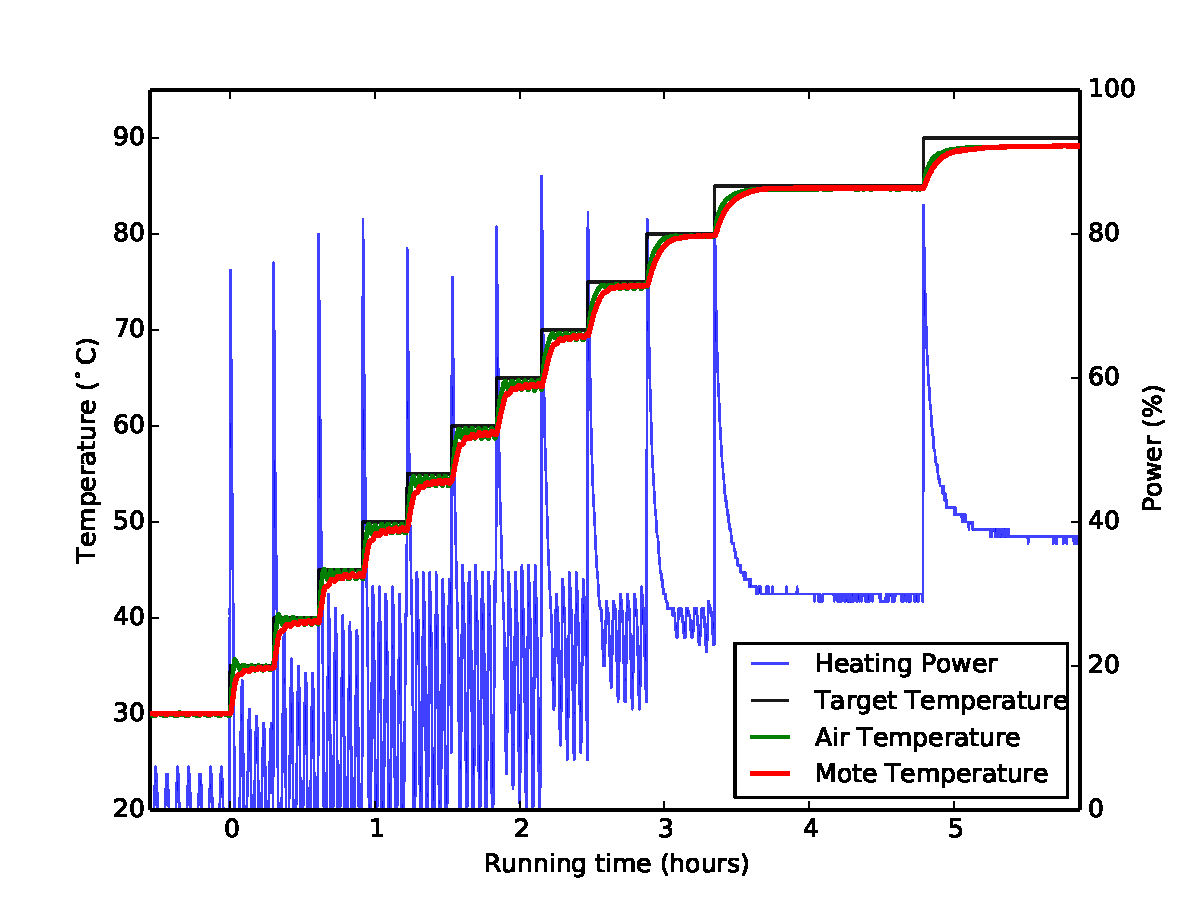
\includegraphics[width=0.475\columnwidth]{figures/box_heating_step}
	    \label{fig:box_heating_step}
	}
	\caption{Typical performance of the boxes over time. Notice the mote temperature (red line) lagging behind air temperature (green line).}
	\label{fig:box_heating_curves}
\end{figure}

Compared to TempLab by Boano~\etal~\cite{Boano2014}, which uses infrared heat lamp controlled via the wireless Z-Wave home automation protocol, our boxes require more manual assembly, do not operate wirelessly and cannot change temperature as fast.
However, our boxes also only cost one third as much (\EUR{91} versus \EUR{293}).

% \newpage


\section{Mote Harness}
\label{sec:mote_harness}

In order to guarantee that both sender and receiver will not move during experiments a mote harness was developed and laser cut out of acrylic.
The mote snaps into the harness so that the axis of rotation goes through the middle of the PCB antenna which then allows rotation in \SI{5}{\degree} steps as shown in Figure~\ref{fig:mote_harness}.
Furthermore, the distance between two harnesses can be adjusted in \SI{5}{\milli\metre} steps using laser-cut wooden distance bars.

In our experiments this greatly improved the handling of the motes. Where before we used to tape the mote down into position, which was an inaccurate matter at best, we now have a simple and elegant solution.
However, we ended up not actually using the distance bars in most of our experiments, as it was simpler to use antenna orientation to control link quality than distance.
Therefore, in Figure~\ref{fig:box_hardware_picture} the mote harness is fixed onto the baseplate.

\begin{figure}[t]
	\subfigure[Harness with mote on a distance bar.] {
		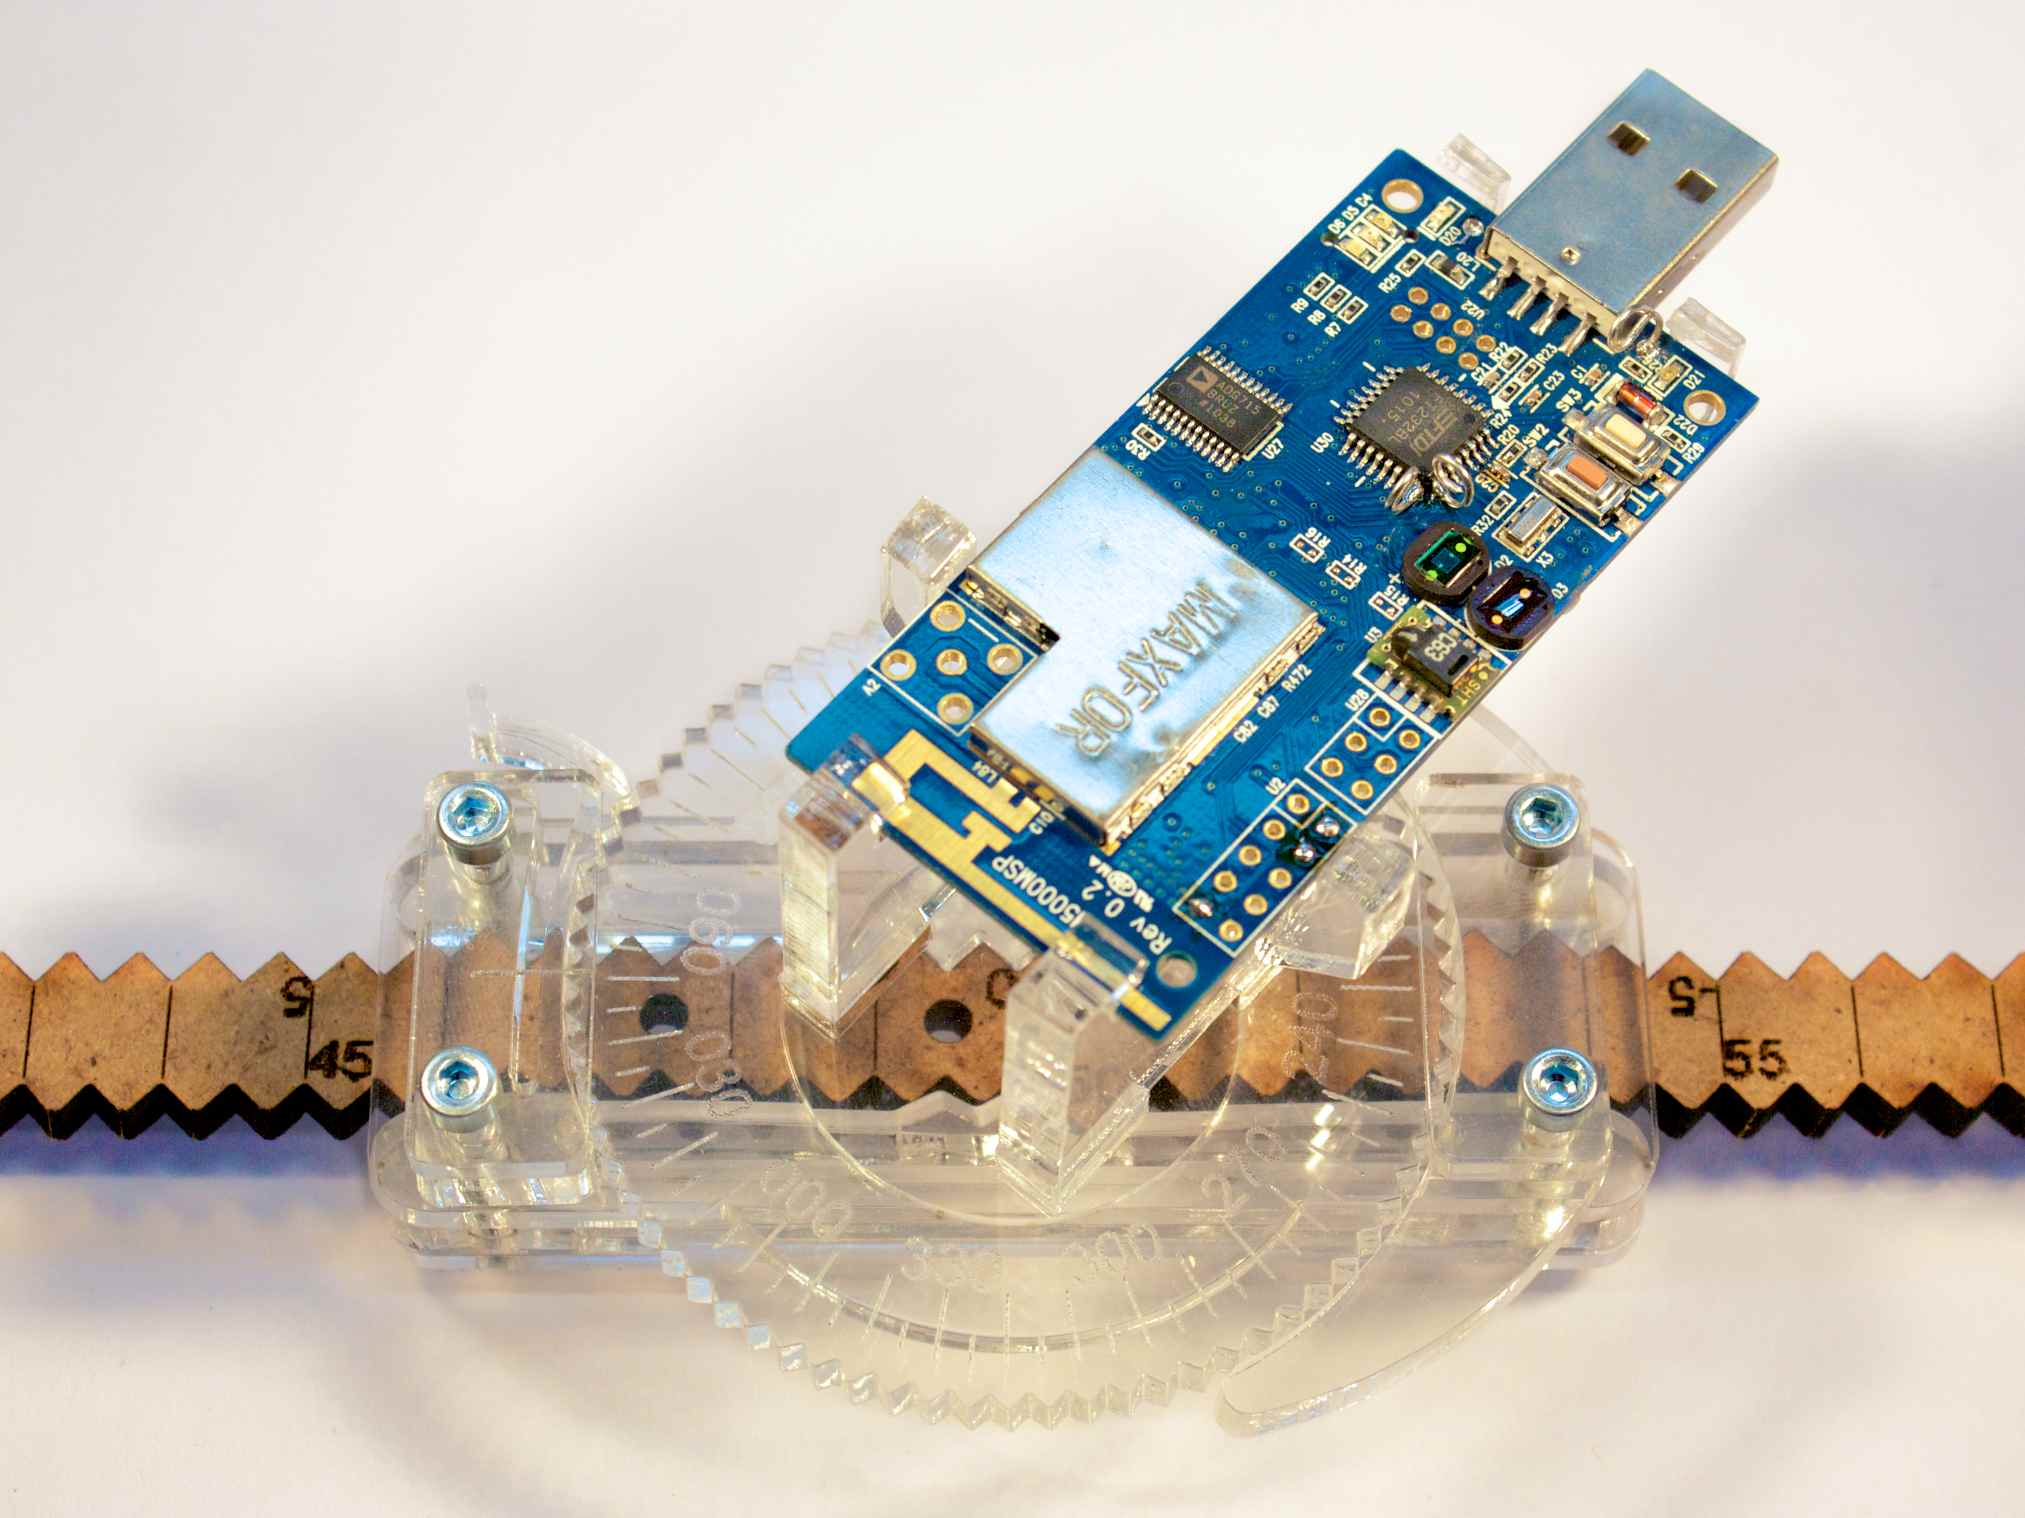
\includegraphics[width=0.5\columnwidth]{figures/harness_picture}
		\label{fig:harness_picture}
	}
	\subfigure[Vector drawing of the rotation disc.] {
		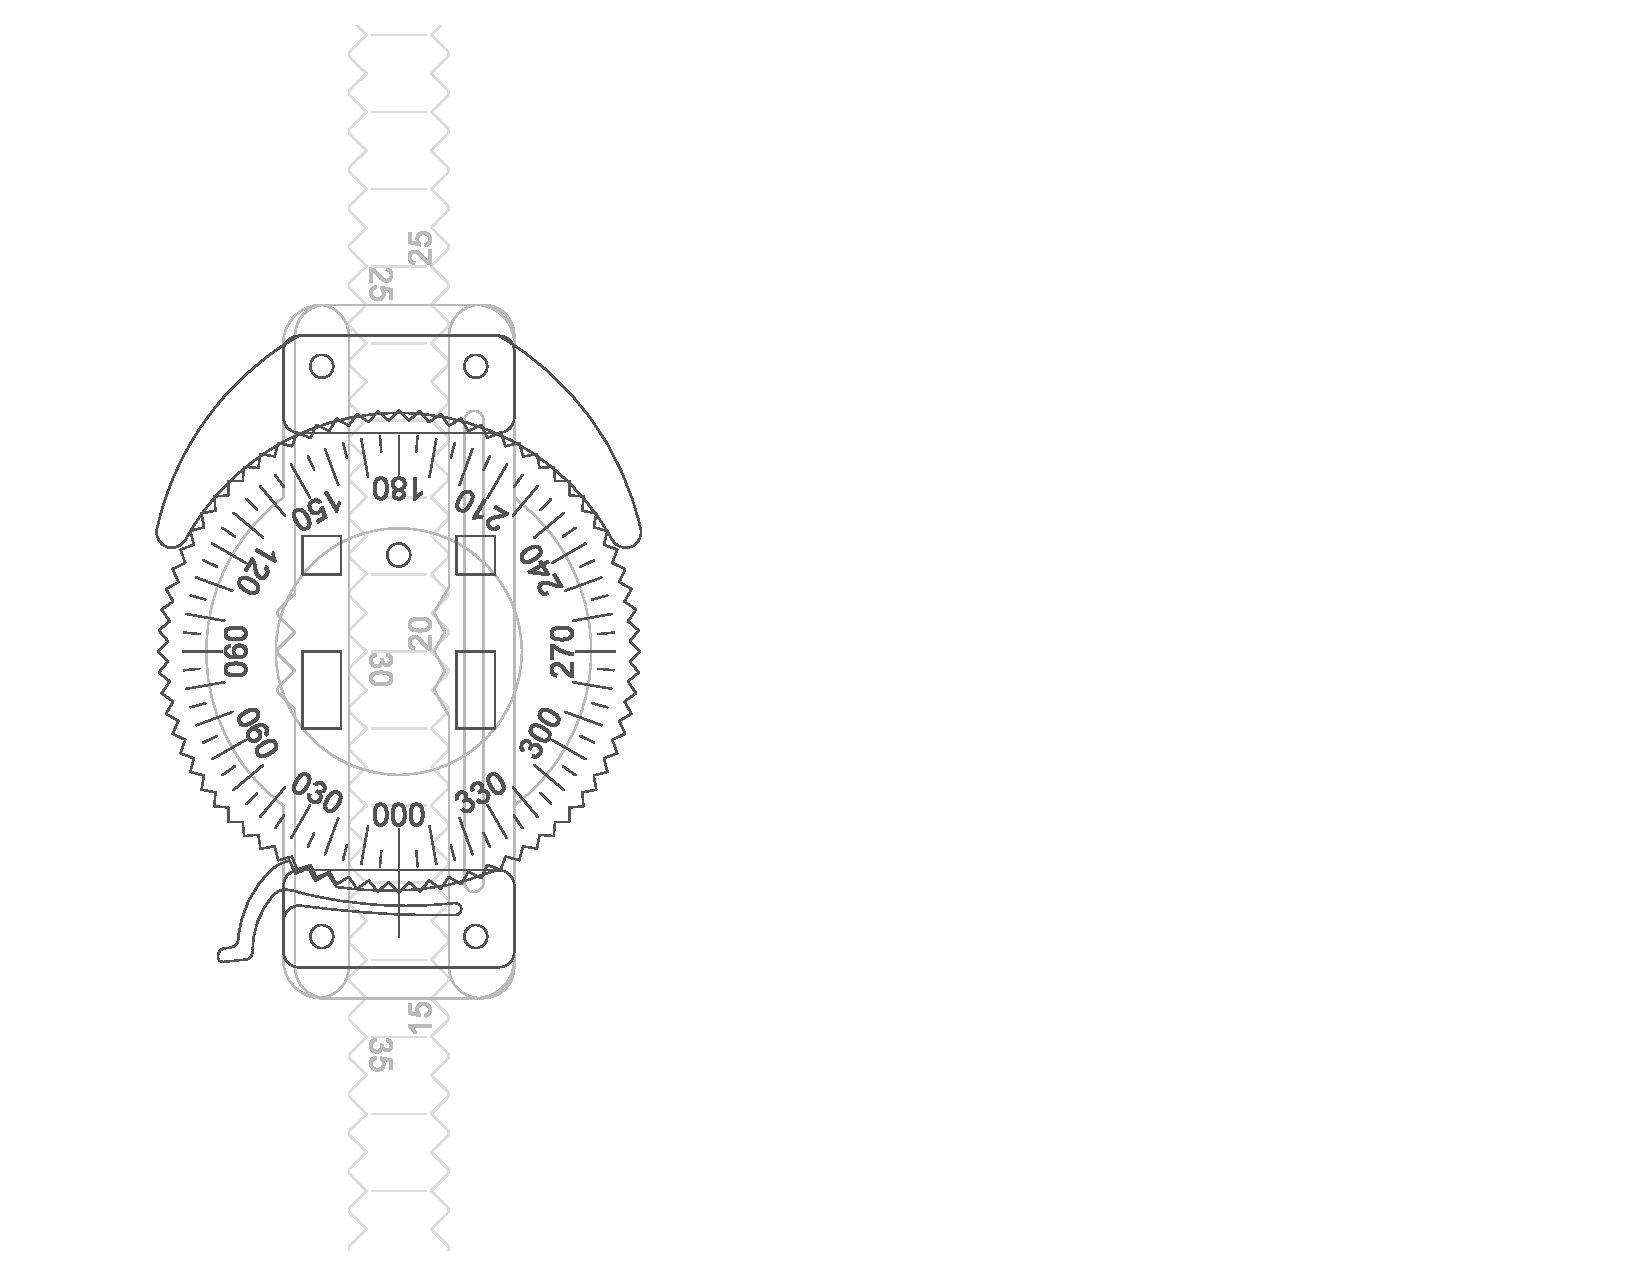
\includegraphics[trim = 20mm 40mm 140mm 45mm, clip, width=0.5\columnwidth, angle=90, scale=0.75]{figures/harness_vector_bar_2}
		\label{fig:harness_vector}
	}
	\caption{The mote harness allows precise positioning of motes.}
	\label{fig:mote_harness}
\end{figure}

% \newpage


\section{Control Software}
\label{sec:control_software}

The motes and temperature boxes are connected via USB-to-Serial converters to a computer, and controlled with a Python program using the TinyOS Python SDK~\cite{tinyos.net}.
Since all motes are connected to one computer, packet loss due to colliding transmissions is avoided via central scheduling of transmissions.
The software holds virtual representations of the mote, temperature controller and link, and logs experiment results to disk.
A simple scripting language allows the definition of commands that are interpreted by the runtime and executed serially so that experiments can be described in independent and compact form.
Multiple scripts can be added, so that experiments can run unsupervised around the clock.

During an experiment all transmissions and receptions are written to a log in ASCII format, which includes a timestamp, sending and receiving node ids, a sequence number, link quality metadata, mote temperature and the entire \ac{MPDU} payload, including \ac{FCS}.%, as shown in Listing~\ref{lst:log_example}.
These logs describe the entire experiment in a unprocessed format, which is then read by the evaluation scripts that reassemble them into messages and links.

This modular software setup allows for a lot of freedom when designing these experiments, as all evalutation data is based upon these unprocessed logs.
This enables us to use one experiment for multiple purposes by focusing on different parameters, of which we will make use later in in Chapter~\ref{chap:forward_error_correction}.

\begin{listing}[t]
\begin{lstlisting}[breaklines=true]
timestamp=2014-05-03 09:22:21,752	mode=tx	id=0	seqnum=0	temperature=29.9	length=93	data=[...]	power=3
timestamp=2014-05-03 09:22:21,753	mode=rx	id=1	seqnum=0	temperature=33.0	timeout=1

timestamp=2014-05-03 09:22:21,890	mode=tx	id=1	seqnum=1	temperature=33.0	length=93	data=[...]	power=3
timestamp=2014-05-03 09:22:21,890	mode=rx	id=0	seqnum=1	temperature=29.9	length=93	data=[...]	rssi=-90	lqi=104 crc=1 timeout=0
\end{lstlisting}
\caption{A log excerpt showing two transmissions, of which the first reception timed out. The raw data field is ommited for clarity.}
\label{lst:log_example}
\end{listing}


\chapter{Experiment Results}
\label{chap:experiments}

This chapter describes the experiment setups we designed to focus on the effect of temperature on the mote hardware and link quality.
We present the evaluation of the experiment results and compare them to related work.

\section{Locations}

We executed these experiments in two locations: a temperature-controlled server room in a basement and a large empty storage space.
We chose these locations for their low visitation frequency, since the presence of moving objects, especially humans, alters the link quality, which of course was undesirable.

In the server room, a space of about \SI{3 x 12}{\metre} was available, with a thick load-bearing concrete wall on the one side and metallic server racks on the other.
This environment made for a very good link quality even at low power, which was the opposite of what we needed.
We tried a power setting of 3 (\SI{-25}{\dBm}), but even at the maximum attainable distance in the room the link was without bit errors, therefore we settled on power setting 2 (below \SI{-25}{\dBm}), which required the motes to be very close to each other at about \SI{30}{\centi\metre}.
Due to the difficulty of manipulating link quality with fine granularity, we only ran one experiment in this room and then relocated the setup.

The storage room was larger with about \SI{10 x 15}{\metre} and had a window front and many shelves on the walls.
Here we could use power setting 3 at about \SI{3}{\metre} distance and very accurately manipulate link quality.
Therefore we used this location for the remaining experiments.

\section{Desired Link Quality}
\label{sec:link_quality}

To create a link with the desired quality, we used a simple, live updated graphical display of \ac{LQI}, \ac{RSSI} and bit error values.
While links of intermediate quality are relatively easy to find, we found it difficult to find the right intermediate link quality with a high enough \ac{BER} for statistically significant results, but with also enough average message receptions, especially for a longer period of time.
These temporal characteristics have also been described by Baccour~\etal~\cite{Baccour2012}, specifically, that links of moderate average \ac{PRR} are less stable than with very low or very high \ac{PRR}.
Furthermore, the mere presence of a person in the same room as the motes caused a dramatic change in link quality, which has also been described by Baccour~\etal

We briefly considered using a controllable source of radio interference as proposed by Boano~\etal~\cite{Boano2009} to be able to make it easier to create the desired link qualities, however, its effect on the \ac{BER} patterns is unknown and we did not want to risk a corruption of our test results.
Therefore, finding and verifying the desired link quality with the acceptable amount of bit errors regularly took hours, especially when the motes where to be heated to different temperatures.
Even then, we had to repeat several experiments when link quality inexplicably changed.
An automated link quality ``creator'' using a motorized mote harness would certainly have helped.

All experiments were done using the on-board PCB antenna sending on channel 26, which is outside the allotted spectrum of 802.11, to minimize WiFi interference~\cite{Liang2010}.


\section{Microcontroller Clock Drift}
\label{sec:clock_drift}

The Tmote Sky uses a MSP430 microcontroller clocked by an integrated ring oscillator called the \ac{DCO}.
Since the generated clock frequency varies from chip to chip with temperature and operating voltage, the \ac{DCO} can be fine-tuned in software using a modulation functionality.
During booting, TinyOS calibrates the \ac{DCO} using the external low-current \SI{32.756}{\hertz} watch crystal to generate a more accurate \SI{1}{\mega\hertz} clock.
It should be noted, that by default calibration only occurs after a reset, and not periodically during program execution.

We noticed that serial communication stopped working after heating the nodes above $55-$\SI{60}{\celsius}. Below this temperature the problem could be mitigated by resetting the mote to trigger a recalibration of the \ac{DCO}.
Boano~\etal{} reported similar synchronization trouble in their TempLab setup~\cite{Boano2014}.
We therefore looked at the output of the \ac{UART} module with a logic analyzer and measured how the selected baudrate changed over temperature.
The \ac{UART} receiver can tolerate up to $\pm5\%$ relative error, however, with the relative errors of several baudrates reaching well over $-20\%$ as shown in Figure~\ref{fig:baudrate_error}, resynchronization is impossible.

Since the baudrate is generated by scaling the \ac{DCO}, the \emph{relative} baudrate error is equivalent to \emph{relative} \ac{DCO} error over temperature.
We calculated an average temperature clock drift coefficient of \SI{-0.367}{\%\per\celsius}, which is within the typical range according to the datasheet. Similar coefficients were found by Z{\'u}{\~n}iga~\etal~\cite{Zuniga2013}.

\begin{figure}[t]
	\subfigure[Relative error of four baudrates.] {
    	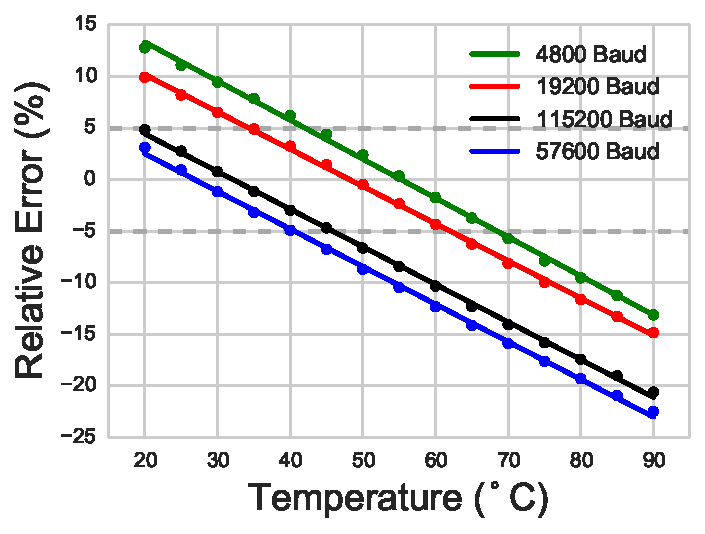
\includegraphics[width=0.475\columnwidth]{figures/baudrate_error}
    	\label{fig:baudrate_error}
    }
    \subfigure[Relative error of \acs{DCO} calibration.] {
	    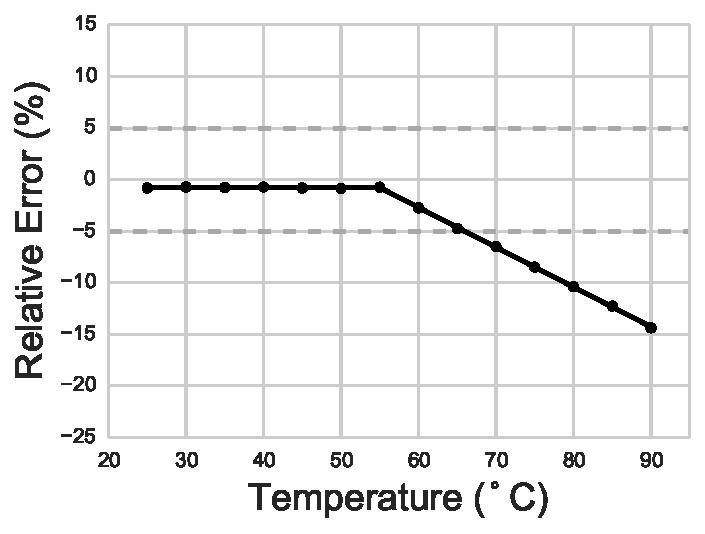
\includegraphics[width=0.475\columnwidth]{figures/reboot_dco_drift}
	    \label{fig:reboot_drift}
	}
	\subfigure[Relative error of corrected baudrate.] {
	    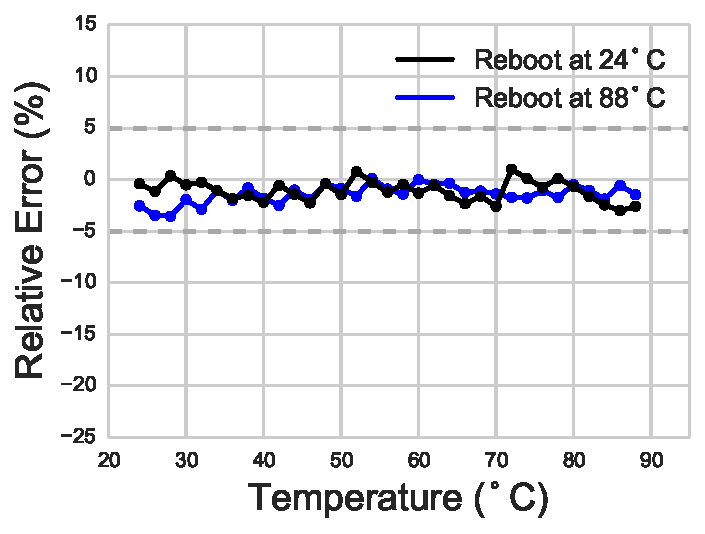
\includegraphics[width=0.475\columnwidth]{figures/baudrate_correction_error}
	    \label{fig:baudrate_look_up_error}
	}
	\subfigure[Values of baudrate correction look-up table.] {
	    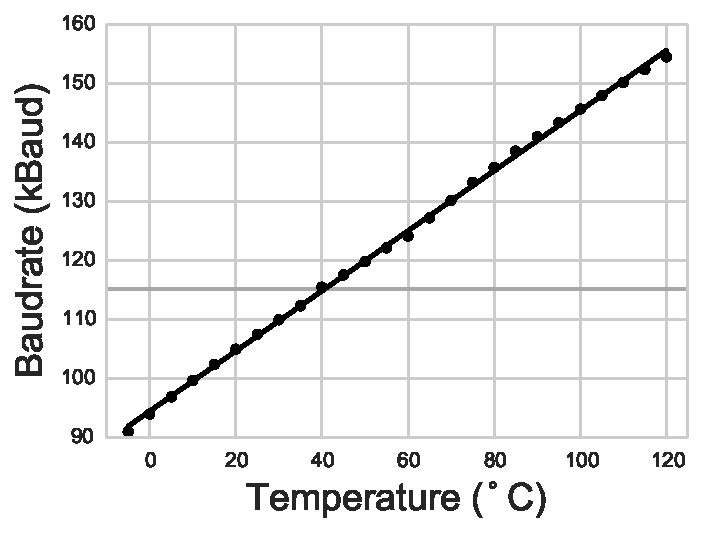
\includegraphics[width=0.475\columnwidth]{figures/baudrate_correction_table}
	    \label{fig:baudrate_look_up}
	}
	\caption{\acs{UART} and \acs{DCO} calibration errors over temperature. The dotted gray line indicates $\pm5\%$ \acs{UART} tolerance.}
\end{figure}

We then measured the relative baudrate error after rebooting over temperature.
As shown in Figure~\ref{fig:reboot_drift}, the TinyOS implementation of the \ac{DCO} calibration only works until \SI{55}{\celsius}, after which it has no corrective effect on CPU frequency, making periodic \ac{DCO} calibration during program execution ineffective.
It is possible that Contiki OS~\cite{contiki-os.org} does not experience these problems as their \ac{DCO} calibration algorithm is different from TinyOS. We did not test this, however.

To not influence the operation of the rest of the microcontroller and since understanding the \ac{DCO} calibration algorithm is not the focus of this thesis, we chose not to correct \ac{DCO} drift directly, but counteract only its effect on baudrate.
To stay within the required tolerance of $\pm5\%$ relative error, we created a fixed lookup-table of ``inverse'' correction baudrates for 115.2kBaud as shown in Figure~\ref{fig:baudrate_look_up}.

Since calculation of prescaler values at runtime is very costly (requiring floating point arithmetic in a recursive algorithm) the look-up table only contains precalculated values, which are then copied into the registers at runtime.
The on-board sensor provides temperature to the \ac{UART} module, which then selects new prescaler values from the look-up table for every \SI{5}{\celsius} temperature difference, which shows up as a sawtooth pattern in Figure~\ref{fig:baudrate_look_up_error} of the resulting relative error of the corrected baudrate.

We used this correction table without change on all of our motes and did not encounter this problem again.
This shows that even with slight differences in clock drift coefficient between different motes, this is approach is enough to solve this issue for our study.

Clock drift is not an issue for the communication between the MSP430 and the CC2420, as it is connected via the \ac{SPI}, which is a synchronous master-slave bus that provides the communication clock for its slaves, requiring no synchronisation on data symbols.


\section{Patterns in Bit Error Distributions}
\label{sec:bit_error_patterns}

We designed two experiments to investigate the results of Schmidt~\etal~\cite{Schmidt2013}.
The first experiment was used to confirm their findings and also investigate the influence of hardware layout on \ac{BER} patterns, while the second experiment investigated the influence of temperature on these patterns.

\subsection{Effects of Board Layout}
\label{subsec:effects_of_board_layout}

In all our experiments we used Tmote Sky motes, which are commercial drop-in replacements for the original Telos mote design by Polastre~\etal~\cite{Polastre2005}.
We had hardware revisions available from two manufacturers: the original design from (now defunct) MoteIV Corporation and the Maxfor MTM-CM5000MSP, which uses a slightly different schematic and board layout.
Notable differences include the \SI{3}{\volt} regulator and the physical layout of the radio circuitry.

In the experiment a pair of CM5000 and original motes transmitted to two CM5000 and two original motes.
All motes were powered by the on-board voltage regulator via the USB connector, which was also used to establish serial communications with the PC.
This redundant placement shown in Figure~\ref{fig:8mote_experiment_setup} was chosen so that the same transmission was received by both types.
Over the course of six days the four transmitters sent 563,500 messages each, totaling 2,254,000 transmitted messages at power setting 2 (below \SI{-25}{\dBm}).
Since each transmission was sent to four receivers, a total of 9,016,000 receptions should have been possible.
Of those 5,280,369 were received and 2,497,744 had at least one bit error.
The experiment was located in the large climate-controlled server room in the basement, where the temperature remained within $20$--\SI{25}{\celsius} with no other changes in the environment.

\begin{figure}[t]
	\centering
	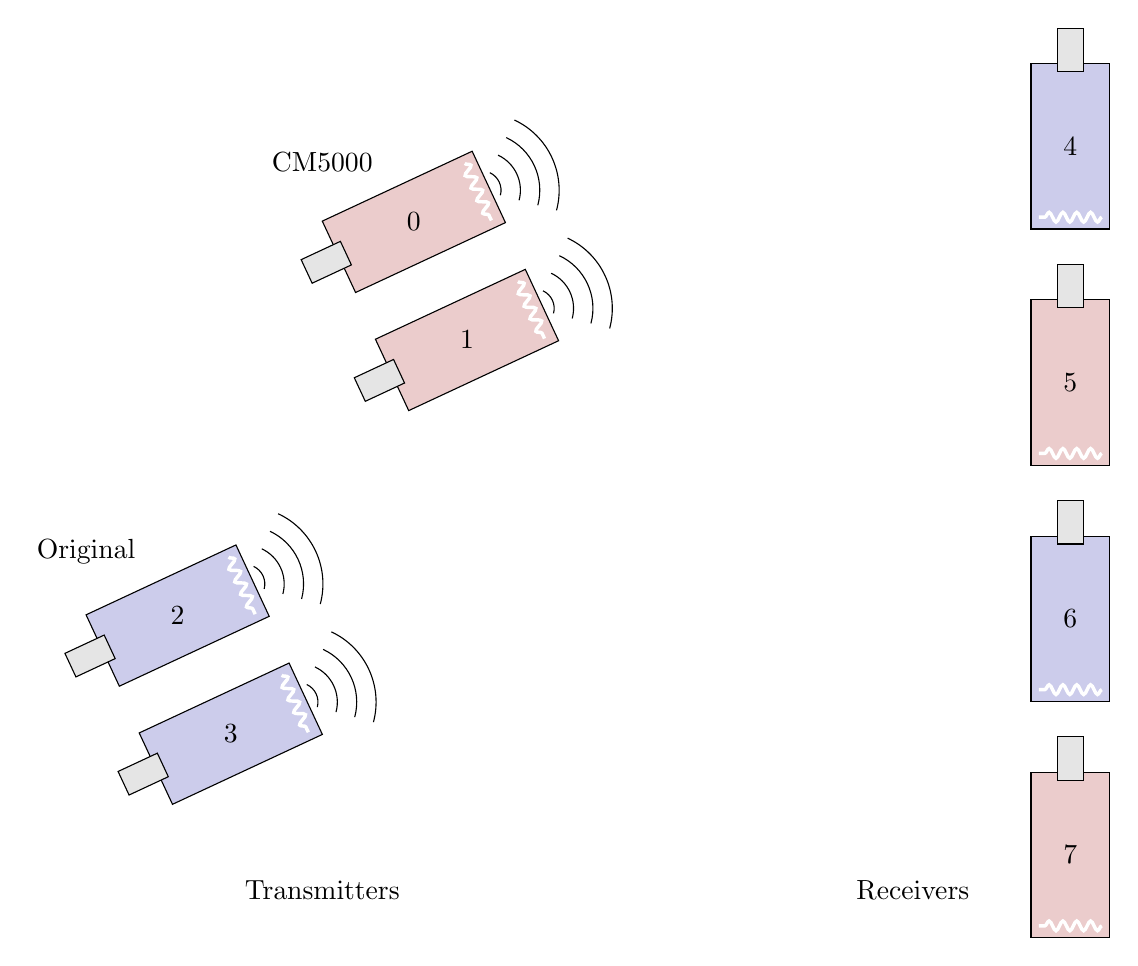
\begin{tikzpicture}
		\newcommand\receiver[5]{%
		    \begin{scope}[xshift=#1cm,yshift=#2cm,rotate=#3]
		        \draw[fill=#4] (0,0) rectangle (1,2.1);
		     	\draw[fill=black!10] (0.33,0.1) rectangle (0.66,-0.45);
		     	\draw[snake=snake, white, segment amplitude=1.75, segment length=5, line width=1.25pt] (0.1, 1.95) -- (0.9, 1.95);
		     	\node at (0.5cm, 1.05cm) {#5};
		    \end{scope}
		}
		\newcommand\transmitter[5]{%
			\receiver{#1}{#2}{#3}{#4}{#5};
		    \begin{scope}[xshift=#1cm,yshift=#2cm,rotate=#3]
		     	\draw[snake=expanding waves, segment angle=40, segment length=7] (0.5,2) -- (0.5,3);
		    \end{scope}
		}

		% new = red, old = blue
		% new transmitter
		\transmitter{3}{7}{-65}{motered}{0};
		\transmitter{3.675}{5.5}{-65}{motered}{1};		

		% new transmitter
		\transmitter{0}{2}{-65}{moteblue}{2};
		\transmitter{0.675}{0.5}{-65}{moteblue}{3};

		\receiver{13}{0}{180}{motered}{7};
		\receiver{13}{3}{180}{moteblue}{6};
		\receiver{13}{6}{180}{motered}{5};
		\receiver{13}{9}{180}{moteblue}{4};

		% labels
		\node at (3, 7.75) {CM5000};
		\node at (0, 2.8) {Original};

		\node at (3, -1.5) {Transmitters};
		\node at (10.5, -1.5) {Receivers};
	\end{tikzpicture}
	\caption{Experiment setup with four transmitters and four receivers.}
	\label{fig:8mote_experiment_setup}
\end{figure}

The CM5000 motes required to be physically closer to the receivers at the same power setting to have similar link quality as the original motes.
This might be hinting at a difference in range between the two hardware layouts, however, our experiment was not set up to systematically investigate range.

In the initial evaluation we noted some significant differences in the quality of some links, where the co-located transmitters are sending to the same receiver.
For example, the link 3--5 is of very good quality with over 99\% \ac{PRR}, however link 2--5 shows quite the opposite with less than 1\% \ac{PRR}, even though both transmitters are located at the same distance and angle from the receiver.
This confirms the findings of Baccour~\etal~\cite{Baccour2012}, specifically that link quality is anisotropic, \ie the communication range exhibits a non-spherical pattern.
More exhibitions of this behavior can be found in the complete table of link qualifiers in the Appendix as Table~\ref{tab:8mote_link_qualities}.

Further analysis revealed the same bit and symbol error patterns as first discovered by Schmidt~\etal~\cite{Schmidt2013}, which state that within any transmitted symbol, the first three \acp{MSB} are more likely to break than the \ac{LSB} and that symbols 8--15 with the \ac{MSB} set to 1 are more likely to break than 0--7.
The normalized occurance of bit errors are plotted in Figure~\ref{fig:8mote_bit_errors}, with the first 12 bytes (96 bits) consisting of the message header with partially fixed content and the remaining 80 bytes are the constant payload, made up of two 32 byte patterns of 0x0000, 0x1111, $\ldots$ 0xFFFF, and one 16 byte pattern of 0x00, 0x11, $\ldots$ 0xFF.

\begin{figure}[t]
	\subfigure[XL] {
    	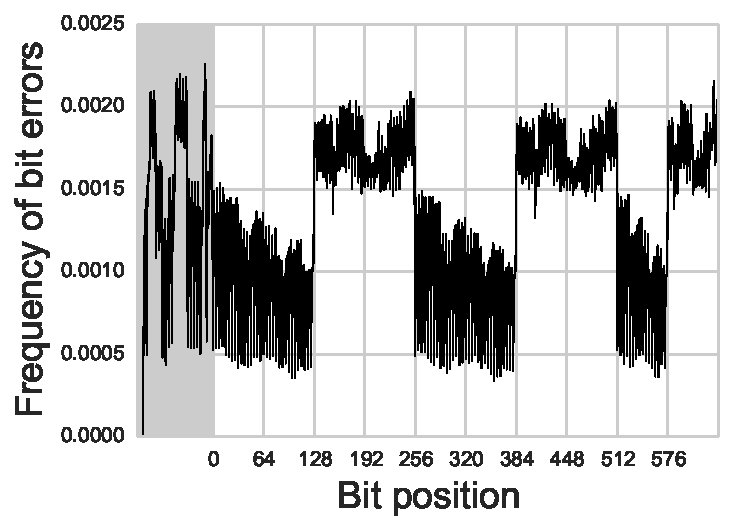
\includegraphics[width=0.475\columnwidth]{figures/8mote_0-5_xor}
    	\label{fig:8mote_bit_errors_xl}
    }
    \subfigure[L] {
	    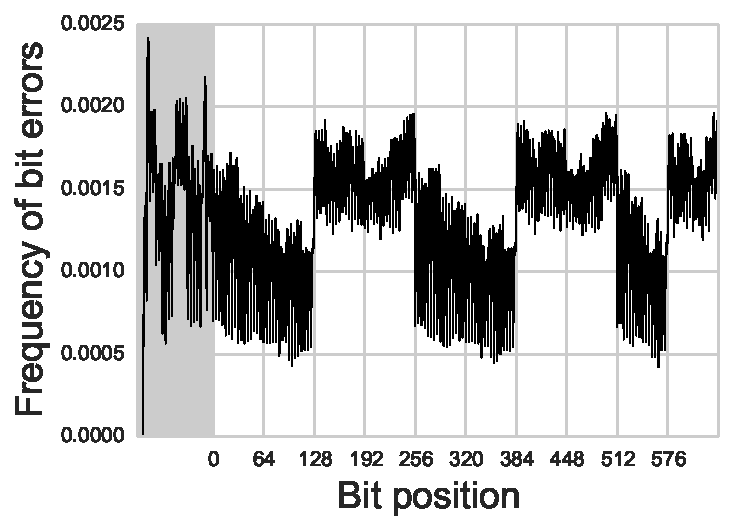
\includegraphics[width=0.475\columnwidth]{figures/8mote_1-6_xor}
	    \label{fig:8mote_bit_errors_l}
	}
	\subfigure[M] {
	    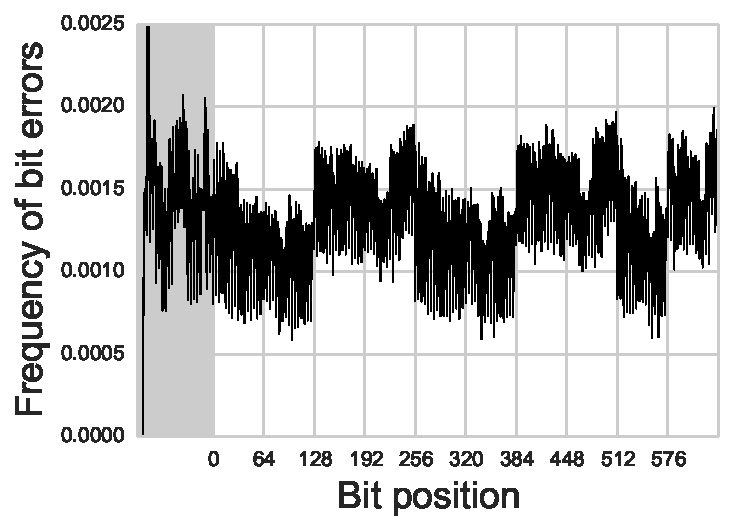
\includegraphics[width=0.475\columnwidth]{figures/8mote_2-6_xor}
	    \label{fig:8mote_bit_errors_m}
	}
	\subfigure[S] {
	    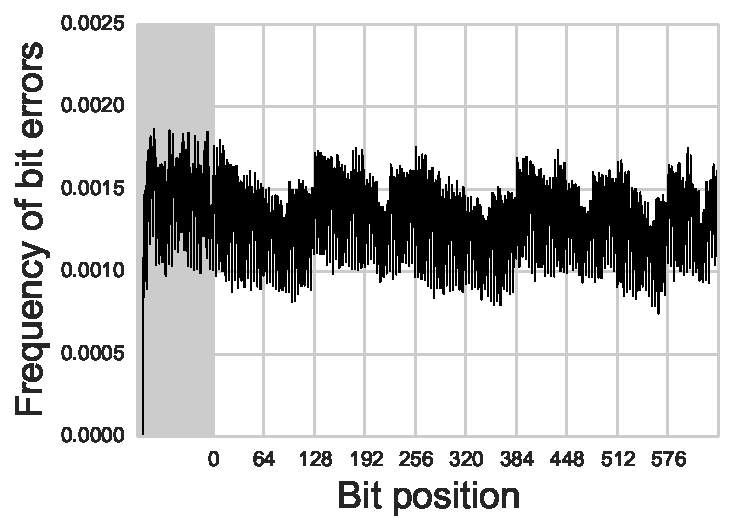
\includegraphics[width=0.475\columnwidth]{figures/8mote_2-7_xor}
	    \label{fig:8mote_bit_errors_s}
	}
	\caption{Four magnitudes of \acs{BER} patterns with fixed payload of twice 0x0000, 0x1111, $\ldots$ 0xFFFF and once 0x00, 0x11, $\ldots$ 0xFF. The message header is indicated in gray.}
	\label{fig:8mote_bit_errors}
\end{figure}

We were able to confirm the findings of Schmidt~\etal{} and extend them with a classification of the influence of symbols on \ac{BER}.
The Subfigures in \ref{fig:8mote_bit_errors} show four magnitudes of this phenomenon, ranging from an extreme to almost no difference between symbols, named XL, L, M and S.
The remaining links can be classified into these four categories as done in Table~\ref{tab:8mote_bit_error_link_classification}.
XL and L patterns seems to be more common than M and S, with 8 vs. 3 links respectively, however, the table is incomplete, since only 11 out of 16 links had enough bit errors to recognize and categorize the pattern.

Schmidt~\etal{} also looked into the burstiness of errors and showed in their research that burst errors are not independently distributed.
The authors explained the drop from 4-bit bursts to 5-bit bursts with the added difficulty of corrupting a minimum of 7 bits to overcome the minimum Hamming distance of 12 between two symbol's chip sequences.
They also hypothesized that a similar drop would occur between 8-bit and 9-bit bursts, but were unable to confirm this, due to their limited sample size.
With our larger sample size we can confirm their hypothesis, with the drop quite noticeable in Figure~\ref{fig:8mote_xl_burst}.

\begin{table}[ht]
	\begin{tabularx}{\linewidth}{|c*{4}{|c}|}
	\hline
	\T \cellcolor{slightgray} Receiver	& \multicolumn{1}{X|}{\cellcolor{motered} \centering Sender 0} & \multicolumn{1}{X|}{\cellcolor{motered} \centering Sender 1} & \multicolumn{1}{X|}{\cellcolor{moteblue} \centering Sender 2}	& \multicolumn{1}{X|}{\cellcolor{moteblue} \centering Sender 3}\\
	\hline

	\cellcolor{moteblue}\T 4 & S  & \cellcolor{slightgray} & \cellcolor{slightgray} & \cellcolor{slightgray}   \B\\
	\hline
	\cellcolor{motered}\T  5 & XL & XL & L & XL \B\\
	\hline
	\cellcolor{moteblue}\T 6 & XL & L  & M & \cellcolor{slightgray}   \B\\
	\hline
	\cellcolor{motered}\T  7 & L  & \cellcolor{slightgray} & S & L  \B\\
	\hline 
	\end{tabularx}

	\caption{Classification of all links with enough absolute bit errors (otherwise gray).}
	\label{tab:8mote_bit_error_link_classification}
\end{table}

\begin{figure}[t]
	\subfigure[XL burst error distribution.] {
    	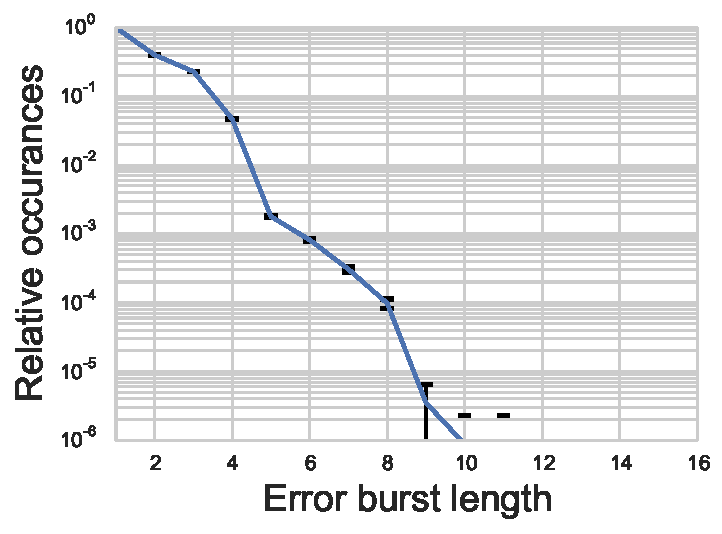
\includegraphics[width=0.475\columnwidth]{figures/8mote_0-5_burst}
    	\label{fig:8mote_xl_burst}
    }
    \subfigure[S burst error distribution.] {
	    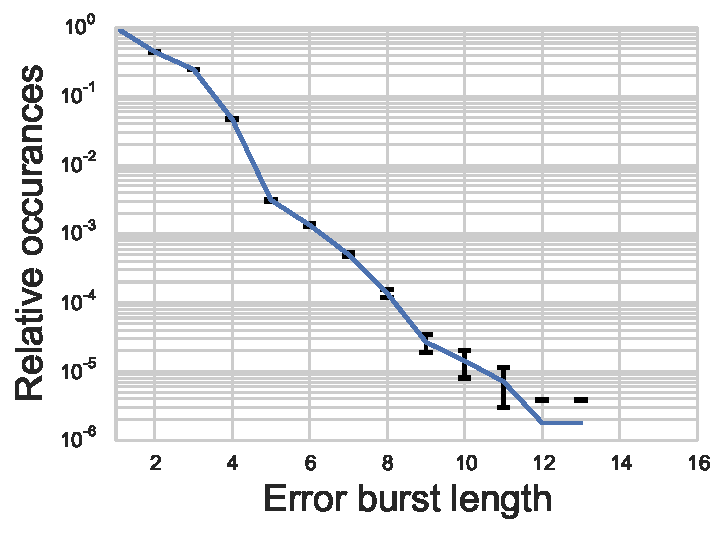
\includegraphics[width=0.475\columnwidth]{figures/8mote_2-7_burst}
	    \label{fig:8mote_s_burst}
	}
	\caption{The burst error distributions of XL and S magnitudes show more longer burst errors in S magnitude. The error bars denote 99\% confidence intervals.}
	\label{fig:8mote_burst_error}
\end{figure}

We cannot see any correlation between the four \ac{BER} pattern classifications and burst error distribution or any other variable.
We therefore believe the magnitude of these patterns to be a result of the analog circuits of the radio, something that cannot be changed or improved by software.

\subsection{Effects of Temperature}
\label{subsec:effects_of_temperature}

To investigate the influence of temperature on \ac{BER} patterns, we used the CM5000 motes in the temperature boxes as described in Section~\ref{sec:temperature_box}.
To minimize signal disturbance we mounted the boxes in the storage room on wooden posts, so that they were floating in free space.
We placed the boxes at a fixed distance of \SI{280}{\centi\metre} to each other and controlled link quality sorely by rotating the antenna.

We ran three experiments with the same constant payload as described in the Subsection~\ref{subsec:effects_of_board_layout} but with power setting 3 (\SI{-25}{\dBm}) at \SI{30}{\celsius}, \SI{50}{\celsius} and \SI{70}{\celsius}.
Due to the decrease of link quality at higher temperatures, discussed in detail in Section~\ref{sec:packet_reception_rate}, we had to adjust mote rotation to regulate \ac{BER} at these temperatures, therefore small differences in absolute bit errors are present.
However, Figure~\ref{fig:temperature_bit_errors} shows no significant difference between \ac{BER} patterns at all three temperatures and therefore we did not pursuit this further.

\begin{figure}[t]
	\subfigure[\acs{BER} pattern at \SI{50}{\celsius}.] {
    	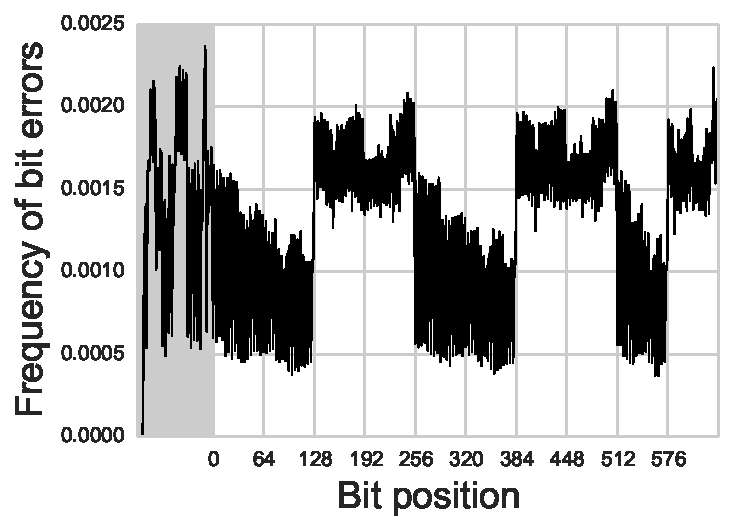
\includegraphics[width=0.475\columnwidth]{figures/temperature_1_5}
    	\label{fig:temperature_bit_errors_30}
    }
    \subfigure[\acs{BER} pattern at \SI{70}{\celsius}.] {
	    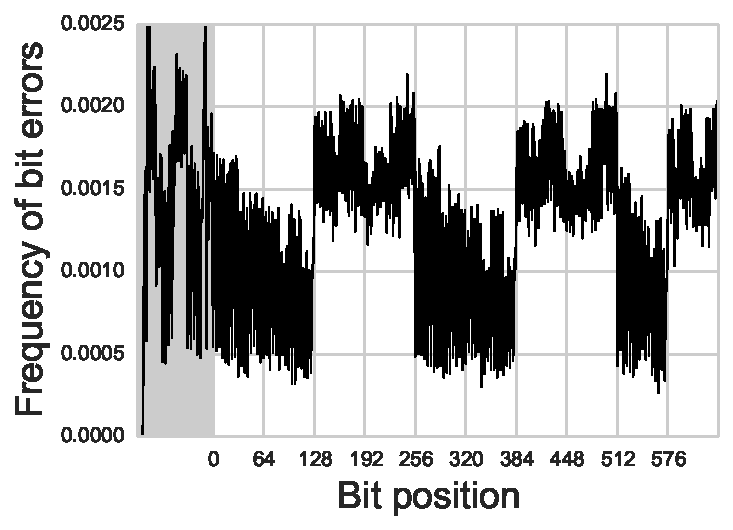
\includegraphics[width=0.475\columnwidth]{figures/temperature_0_6}
	    \label{fig:temperature_bit_errors_70}
	}
	\caption{\acl{BER} patterns show no difference between \SI{30}{\celsius}, \SI{50}{\celsius} and \SI{70}{\celsius}. The pattern at \SI{30}{\celsius} is omitted, since it is redundant.}
	\label{fig:temperature_bit_errors}
\end{figure}


\subsection{Pattern Anomalies}
\label{subsec:pattern_anomalies}

Even though the vast majority of experiment evaluations confirmed these patterns, there were two runs with  drastically different outcome.
We were very surprised to find a second, completely opposite \ac{BER} pattern as shown in Figure~\ref{fig:anomalie_bit_error}.
Here the symbols 0-7 show a higher average \ac{BER} and a less pronounced 4-bit saw-tooth pattern than symbols 8-15.
The pattern almost looks like an ``inverse'' of those described earlier.

The first time it occurred, we attributed this to influences of the environment and discarded it.
Two months later, this pattern occurred again with different hardware in a different setup in a different environment.
Both times, the motes were exposed to high temperature (>\SI{70}{\celsius}) over several hours, however, we were unable to confirm if this indeed triggered the pattern.
This pattern remained for days, regardless of temperature, link quality or message payload.

We cannot envision a source of interference capable of fundamentally changing this \ac{BER} distribution and neither does a permanent change of the radio chip's hardware at high temperature seem possible.
The CC2420 radio is rated to be operated at temperatures up to \SI{85}{\celsius} and to be stored at up to \SI{150}{\celsius}, while our experiments where limited to at most \SI{90}{\celsius} for a few hours.

Since we could not find any other reference to this pattern in literature and due to the rarity of this occurrence in our experiments and the difficulty of its repeatability, we decided to focus on investigating the ``normal'' patterns.

\begin{figure}[t]
	\subfigure[First occurance.] {
    	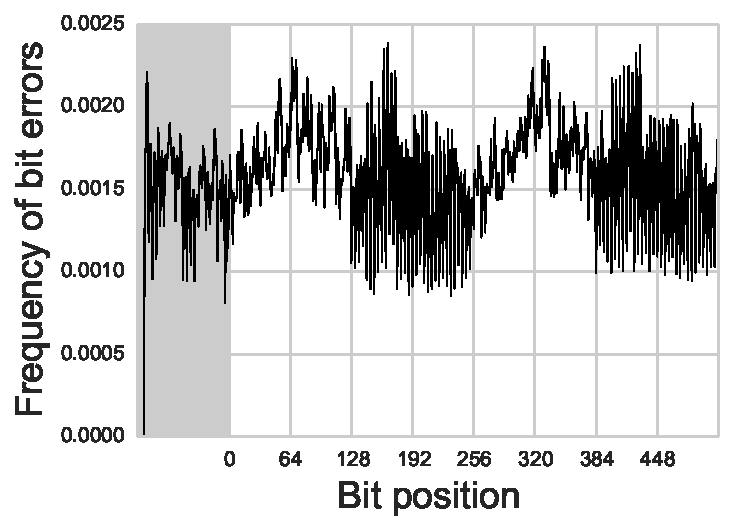
\includegraphics[width=0.475\columnwidth]{figures/anomaly_first}
    	\label{fig:anomalie_earlier}
    }
    \subfigure[Second occurance.] {
	    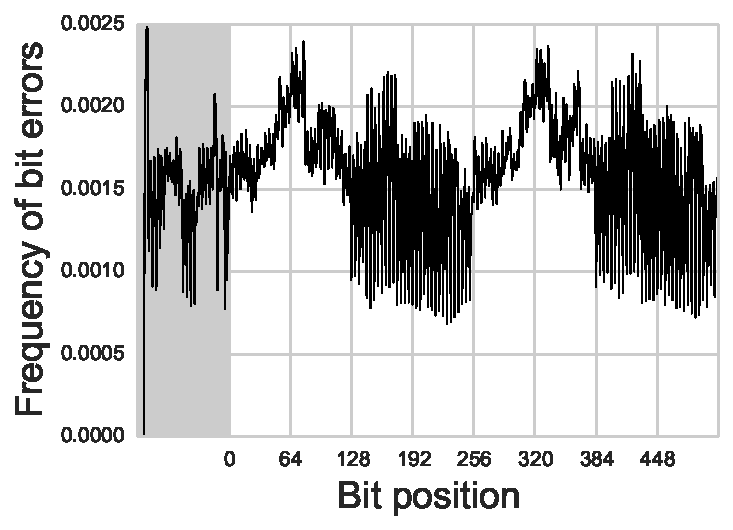
\includegraphics[width=0.475\columnwidth]{figures/anomaly_second}
	    \label{fig:anomalie_later}
	}
	\caption{``Inverted'' \acs{BER} pattern anomaly of constant data. Only the first two 32 byte patterns are shown.}
	\label{fig:anomalie_bit_error}
\end{figure}




\section{Packet Reception Rate}
\label{sec:packet_reception_rate}

The effect of temperature and other environmental factors on link quality has most thoroughly been investigated with the conclusion that all measurements of link quality deteriorate with higher temperature, as one would expect~\cite{Wennerstrom2013, Boano2013, Boano2014, Zuniga2013}.
However, Boano~\etal{} showed in their experiments that this behavior is not symmetrical, since heating the transmitter caused a more significant drop in \ac{PRR} than heating the receiver~\cite{Boano2013}.

In this experiment we used the same physical setup as described in Section~\ref{subsec:effects_of_temperature}, but with random payload as message content.
We fixed mote rotation to create a link that is just starting to deteriorate at \SI{50}{\celsius}, so that at low temperatures the link is of good quality, while at very high temperatures the link will experience high \ac{BER}s.

We increased the temperature of the mote in box 0 in steps of \SI{5}{\celsius} and \SI{10}{\celsius} up to \SI{80}{\celsius} and kept the mote on box 1 at constant \SI{30}{\celsius}, while sending 180.000 messages back and forth.
Then we repeated this, but heated box 1 and kept box 0 temperature constant.
To cancel out environmental factors we ran this experiment four times over two days, so we could then pick the two results with the least interference.

For the evaluation we plotted the normalized \ac{PRR} of messages sent from one mote and received by the other mote over temperature and time and included \ac{BER} and \ac{LQI} and \ac{RSSI} values to illustrate link quality.
Figure~\ref{fig:prr_link_01} shows messages sent from mote 0 addressed to mote 1 for both temperature cycles, while Figure~\ref{fig:prr_link_10} shows the opposite direction.
It becomes immediately clear that a higher temperature of either transmitter or receiver makes the link quality worse, validating the findings of Boano~\etal{} and Wennerstr{\"o}m~\etal~\cite{Boano2013, Wennerstrom2013}.
However, this relationship is neither linear nor symmetrical.


\subsection{Effects of Temperature on \acs{PRR} and \acs{BER}}

In Figure~\ref{fig:prr_link_01} the decrease in \ac{PRR} is small and relatively symmetrical up to about \SI{65}{\celsius}, however, past that point we see a dramatic change, with the increments in temperature translating very strongly into significant drops in \ac{PRR}.
The drop in \ac{PRR} is not symmetrical and becomes much more pronounced, when the receiver is heated than when the transmitter is heated, especially visible in the last increment from \SI{70}{\celsius} to \SI{80}{\celsius}.

This asymmetry is even more extreme in link 1-0, shown in Figure~\ref{fig:prr_link_10}, where heating the receiver beyond \SI{70}{\celsius} will cause an almost complete loss of message reception.
Interesting is the little dip in \ac{PRR} around \SI{50}{\celsius} in Figure~\ref{fig:prr_link_10_receiver}, which was present in this link in all four experiments with varying intensity. We suspect that this is a non-linearity in the radio, cases of which have also been reported by Boano~\etal

The \ac{BER} acts like an inverse function of \ac{PRR}, since higher \ac{BER} yields more messages with at least one bit error.
Noise on \ac{PRR} is visible in the standard deviation of \ac{BER} as exemplified by Figure~\ref{fig:prr_link_10_transmitter}.


\subsection{Effects of Temperature on \acs{LQI} and \acs{RSSI}}

The \ac{LQI} is a very good mirror of the \ac{PRR} of messages without error.
When the receiver is kept at a constant temperature, the values decrease almost linearly with temperature of the transmitter.
This is not the case when the receiver is heated, where a linear correlation to temperature , but is still very similar to the behavior of \ac{PRR}.
We therefore can confirm that \ac{LQI} is a good source for an estimate on \ac{PRR}.

This is very much not the case with \ac{RSSI}, which has much lower resolution that \ac{LQI} and exhibits hysteresis and non-linearities~\cite{Boano2013}.
While in Figure~\ref{fig:prr_link_01}, \ac{RSSI} ends up being lower when the receiver is heated than when it is constant, Figure~\ref{fig:prr_link_10} shows very similar values, even though \ac{PRR} is radically different.

It is also noteworthy that contrary to \ac{LQI}, \ac{RSSI} attempts to describe signal strength (\ie the power level being received by the antenna), which of course does not change, when the transmitter is at constant temperature.
Therefore, without temperature information, the \ac{RSSI} value is misleading, since it represents the power level not at the antenna, but at the signal amplifying stage of the radio. 
Therefore \ac{RSSI} is usable for a very inaccurate estimate of link quality at best, with little to no difference between receiver and transmitter temperature.


\subsection{Discussion}

Our data strongly implicates the receiver as being more vulnerable than the transmitter to an increase in temperature, especially above \SI{65}{\celsius}.
These results are very much incompatible with the findings of Boano~\etal~\cite{Boano2013}, which is surprising since the only two differences between our experiment and theirs is the temperature range and the additional usage of the CC2520~\cite{cc2520} radio, which is very similar to the CC2420~\cite{cc2420}.
However, these differences should not account for completely opposing results.

Research by Bannister~\etal~\cite{Bannister2008} saw an asymmetry in output and received input power when heating transmitter and receiver separately.
At the same time, they measured \ac{PER} and found that above \SI{-90}{\dBm} \ac{RSSI}, temperature had little to no influence, while below that \ac{RSSI} value, \ac{PER} increased.
The authors concluded that the CC2420 \acl{LNA} stage is less efficient at high temperature, which would manifest itself in a significant increase in \ac{PER} (or a \emph{decrease} in error-free \ac{PRR}) on the receiver.
However, the \ac{RSSI} behavior in Figure~\ref{fig:prr_link_10} does not reflect a general truth of the results by Bannister~\etal{} and furthermore suggests no direct correlation between \ac{RSSI} and \ac{PRR}.

We noticed a strong focus in such research on understanding the impact of temperature on output and input signal power, however, it seems that \ac{RSSI} does not actually correspond to link quality in general.
From our data, a combination of \ac{LQI} and temperature seems to have the best correlation to \ac{PRR}, therefore we want to examine how we can use temperature to improve \ac{PRR} in these conditions.

\begin{figure}[t]
	\subfigure[Constant receiver, increasing \newline transmitter temperature.] {
		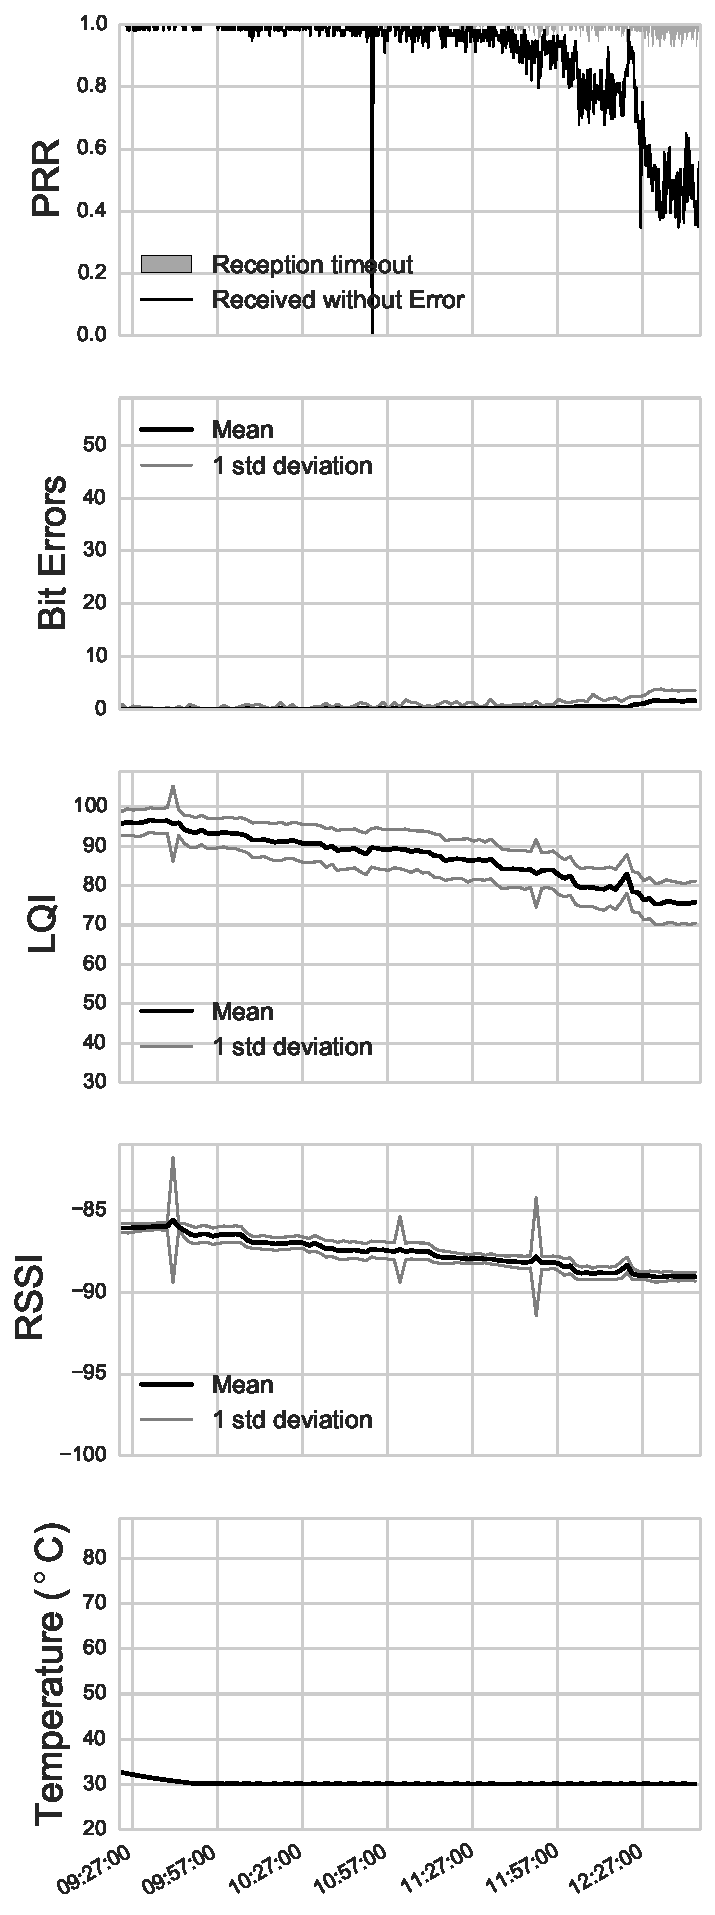
\includegraphics[width=0.475\columnwidth]{figures/prr_0-1_transmitter}
		\label{fig:prr_link_01_transmitter}
	}
	\subfigure[Increasing receiver, constant \newline transmitter temperature.] {
		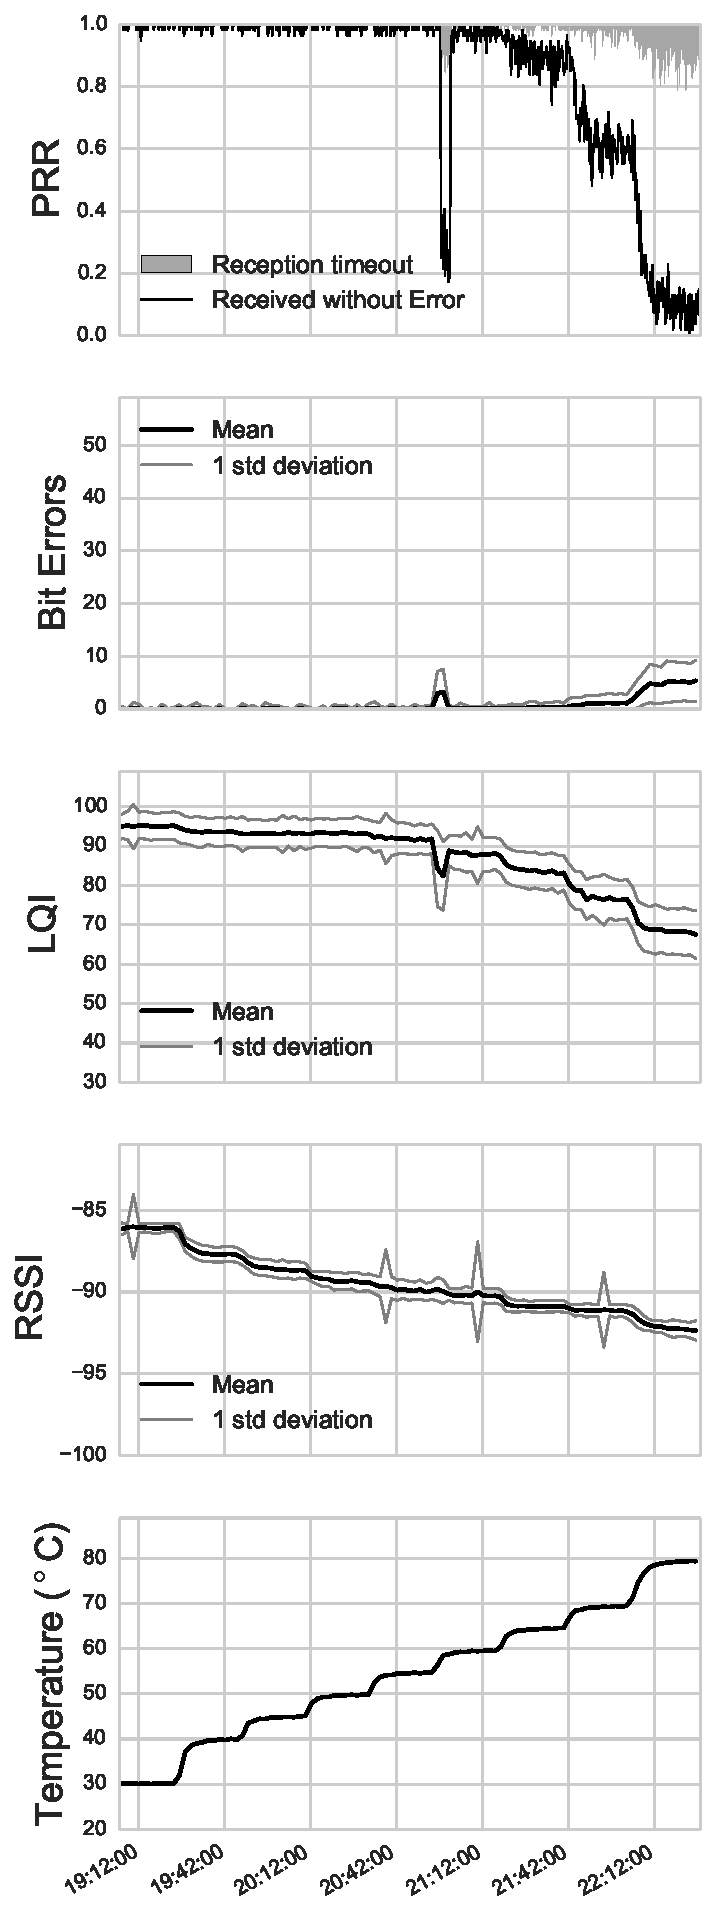
\includegraphics[width=0.475\columnwidth]{figures/prr_0-1_receiver}
		\label{fig:prr_link_01_receiver}
	}
	\caption{\acs{PRR} and link quality of messages received by mote \textbf{1} vs. temperature. For transmitter temperature see Figure~\ref{fig:prr_link_10}.}
	\label{fig:prr_link_01}
\end{figure}

\begin{figure}[t]
	\subfigure[Increasing receiver, constant \newline transmitter temperature.] {
		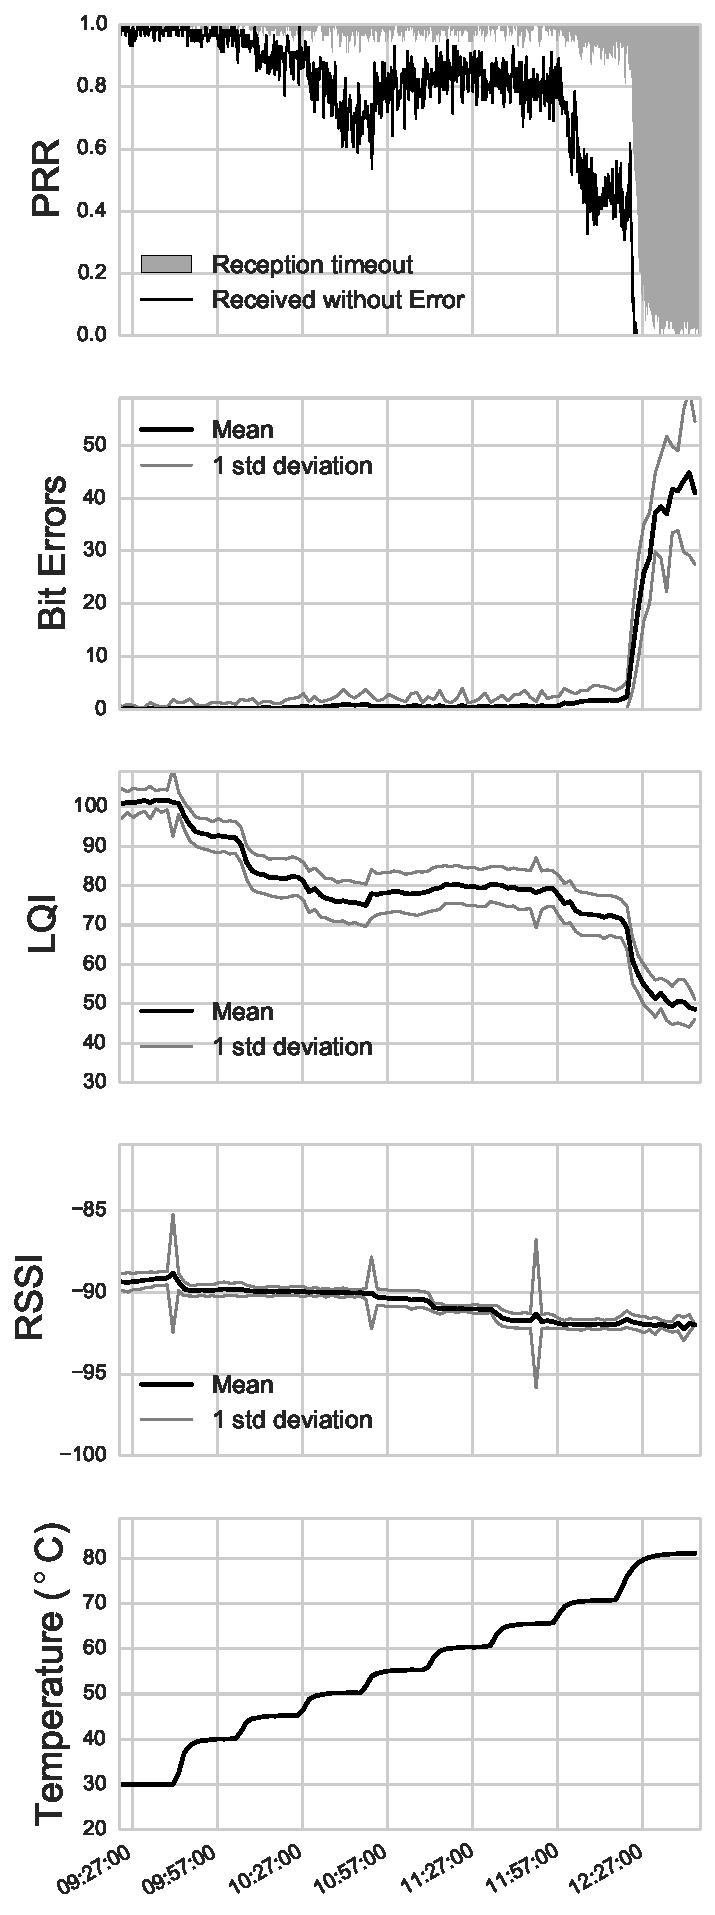
\includegraphics[width=0.475\columnwidth]{figures/prr_1-0_receiver}
		\label{fig:prr_link_10_receiver}
	}
	\subfigure[Constant receiver, increasing \newline transmitter temperature.] {
		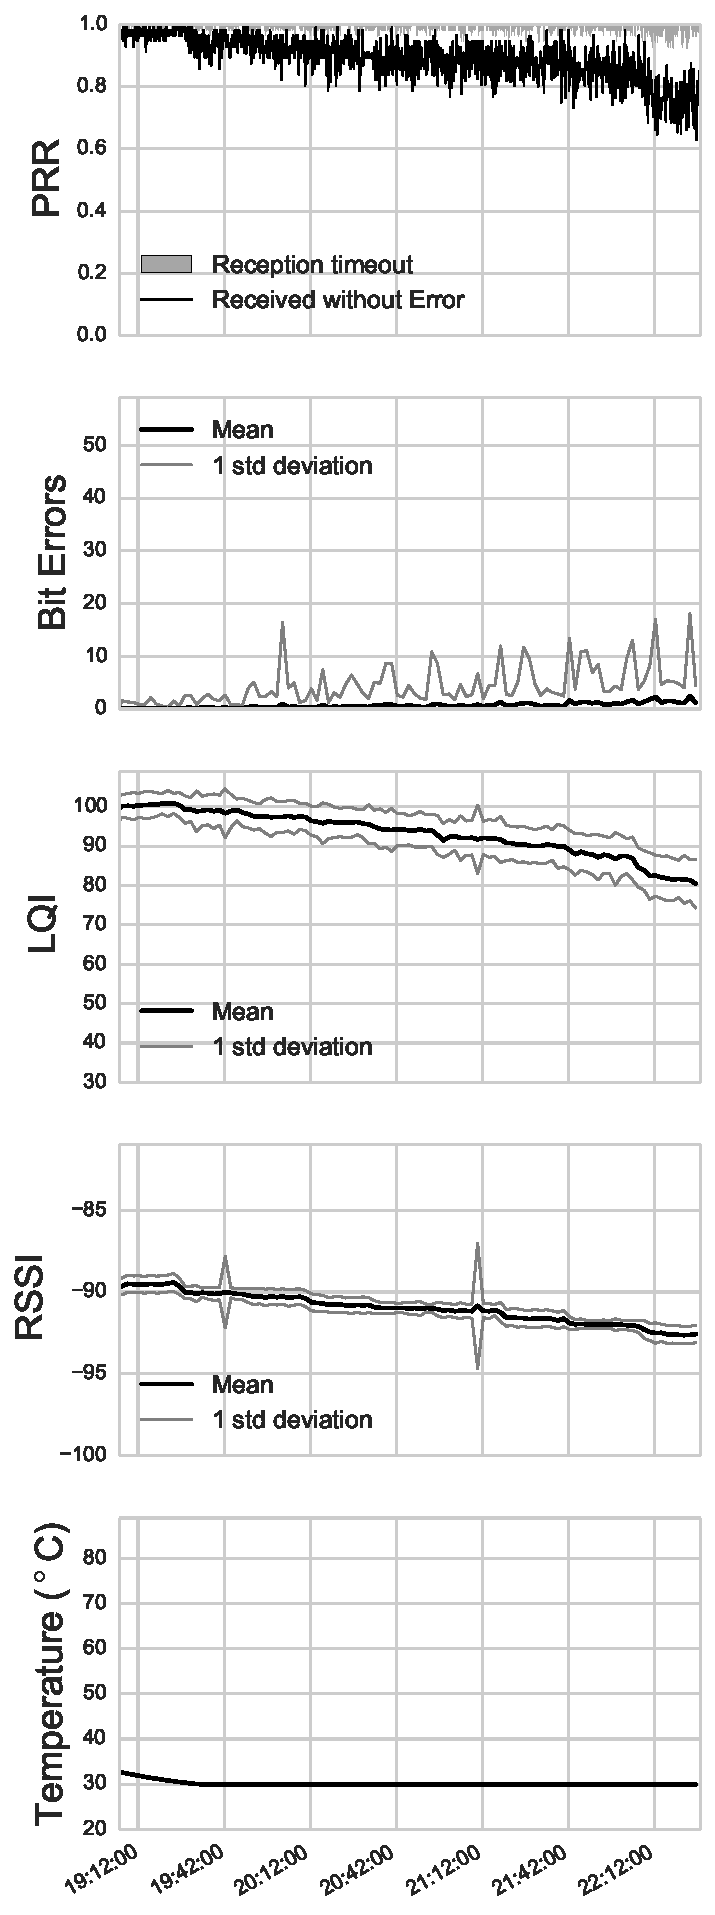
\includegraphics[width=0.475\columnwidth]{figures/prr_1-0_transmitter}
		\label{fig:prr_link_10_transmitter}
	}
	\caption{\acs{PRR} and link quality of messages received by mote \textbf{0} vs. temperature.  For transmitter temperature see Figure~\ref{fig:prr_link_01}. The asymmetry in \acs{PRR} shows much more clearly here.}
	\label{fig:prr_link_10}
\end{figure}



\chapter{\acl{FEC}}
\label{chap:forward_error_correction}

In the last chapters, we described the effect of temperature on \ac{BER} patterns and \ac{PRR}, without drafting any specific recommendations how to improve this loss of link quality.
\ac{FEC} is a well known technique to improve throughput in links of poor quality, however, once a \ac{ECC} and its parameters have been chosen, usually they remain static and do not change over time.
This means that for links where the quality is not stable over time, as in \acp{WSN}, the chosen \ac{ECC} incurs unneeded overhead in links with overal good link quality, and underperforms in links with poor quality.

We therefore wanted to investigate how using temperature as an indicator for adapting \ac{ECC} parameter can benefit \ac{PRR} and throughput and what improvements and limitations to expect.
In doing so, we are moving away from a macro-view of all influences on link quality to focus on the impact of temperature on \ac{FEC} on \emph{one} link at a time.

We extended the control software described in Section~\ref{sec:control_software} to encode messages to be sent and to decode received messages with an \ac{FEC} scheme.
The messages are logged in the same format, with the additional information of the FEC scheme and coding strength.
This allows us to reuse our existing evaluation software to easily map error-free \ac{PRR} to \emph{decoded} error-free \ac{PRR}.


\section{Choice of \acs{FEC} Scheme}

Choosing a coding scheme is not only a matter of its error correction capabilities, but also about the complexity of its coder and decoder, considering the tight computational resources of a \ac{WSN} mote.
Practical implementations are therefore limited to cyclic linear block coding, with the most widely used codes being binary \ac{BCH} and non-binary \ac{RS} codes, which can be combined with interleaving and code shortening~\cite{Liu1997}.
Furthermore, since data payload size is limited to 125 bytes by the \ac{MPDU}, of which we use 93 in our messages (with 80 bytes data), a low coding overhead among \ac{ECC}s with the same error correction capability is preferred.

A \ac{RS} code works over $m$-bit symbols, and is denoted as $RS(n, k)$, where $n$ is the number of $m$-bit symbols in a codeword, and $k$ the number of original $m$-bit data symbols.
This leaves $n-k$ parity $m$-bit symbols, as shown in Figure~\ref{fig:rs_codeword}.
The symbol size $m$ can be set to bit-level, byte-level or packet-level size. We will use byte-level ($m=8$) symbol sizes, since they are efficient to work with on a microcontroller.
A \ac{RS} decoder can correct up to $t=(n-k)/2$ symbol errors, and up to $2t$ erasures, if the positions of the symbol errors are known~\cite{Liu1997}.

Similarly, for symbol size $m \ge 3$ and symbol error occurance $t < 2^{m-1}$, a \ac{BCH} code encodes block lengths of $n = 2^m - 1$ bit with $n-k \le mt$ parity check bits by multiplication with a generator matrix, that contains a $n \times n$ identity and a $n \times (n-k)$ binary matrix.
The decoder can construct a parity matrix using this information, which allows correction of $t$-bit errors, depending on the parameters chosen~\cite{Liu1997}.

Since the \ac{RS} scheme works by correcting entire $m$-bit symbols ($m=8$ for our case), burst errors up to $m$-bit in the same symbol require only correcting this specific symbol, while one-bit errors in many different symbols requires correcting all of these symbols.
\ac{RS} codes therefore perform better than \ac{BCH} codes in conditions with burst errors as described in Subsection~\ref{subsec:effects_of_board_layout}, but worse if same amount of bit errors are spread around more independently.
The performance of \ac{BCH} codes can be improved however, by interleaving symbols after encoding before transmission, which spreads out burst errors into many single bit errors.
However, \ac{BCH} codes generally require more transmission overhead compared with \ac{RS} codes of the same error correction capabilities.

\ac{RS} codes are well understood coding schemes, which have been compared to many others.
By using \ac{RS} codes as a benchmark we enable application of our results onto other, more complex schemes, such as a modified Turbo Code~\cite{Schmidt2009} and \ac{LDPC}~\cite{Sartipi2004} codes, which have been shown to outperform cyclic linear block codes.
Furthermore, a \ac{RS} implementation optimized for TinyOS, called TinyRS~\cite{Liang2010}, exists and therefore does not need to be implemented manually.

\begin{figure}[t]
	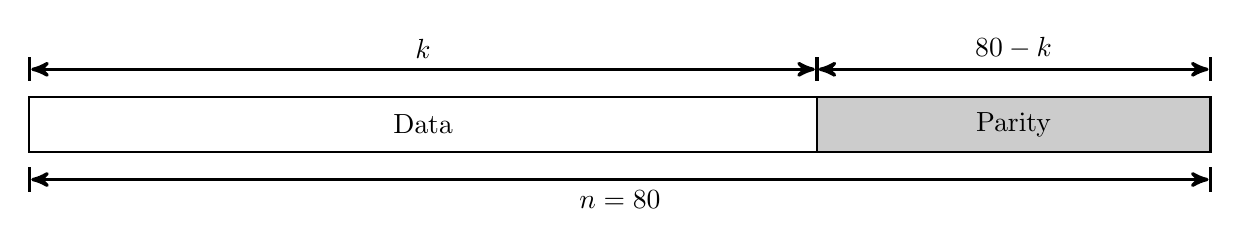
\begin{tikzpicture}[>=stealth', |<->|, very thick, shorten <=-0.5pt, shorten >=-0.5pt]

		\draw[thick] (0,-0.35) rectangle (10,0.35) node[midway] {Data};
		\draw[fill=slightgray, thick] (10,-0.35) rectangle (15,0.35) node[midway] {Parity};

		\draw (0,0.7) -- (10,0.7) node[midway, above] {$k$};
		\draw (10,0.7) -- (15,0.7) node[midway, above] {$80 - k$};
		\draw (0,-0.7) -- (15,-0.7) node[midway, below] {$n = 80$};

	\end{tikzpicture}
	\caption{Structure of an $RS(n, k)$ encoded codeword of 80 bytes length.}
	\label{fig:rs_codeword}
\end{figure}

\section{\acs{RS} Scheme Simulation}
\label{sec:fec_scheme_simulation}

To be able to investigate the effect that different \ac{RS} coding strengths have on decoded \ac{PRR}, we needed a way to compare experiment results.
Due to the difficulty of recreating the \emph{exact} same conditions for several series of real world experiments, we chose to create and use a trace-based simulator to apply the bit error patterns of an original experiment onto several new $RS(n, k)$ encoded random payloads.

By interpreting the $RS(80, 70)$ encoded random payload as pseudo-random in the context of Section~\ref{sec:packet_reception_rate}, we made dual-use of that experiment.
This allows us an in-depth description of the link conditions onto which we built our analysis of \ac{RS} performance.

We will next describe how we use the raw data of this experiment as an input for our simulation, by extracting its \ac{BER} patterns and applying them onto new payload, and discuss accuracy and limitations.

\subsection{Design}

The simulator re-runs an original experiment message-by-message over its log, and outputs a new one.
We only simulate \ac{BER} patterns, all other properties of the link, such as link qualifiers, temperature, transmission power, are copied from the original link, as visualized in Figure~\ref{fig:simulator_design}.
In addition, if a message was not received by a receiver, we simply preserve it as a timeout, to make later comparison of the simulated results with the real experiments much easier.

Our simulator also works with experiments where a transmitted message is received by multiple receivers as in Section~\ref{subsec:effects_of_board_layout}.
In such a case, the simulator will apply its algorithm to every received message.

\begin{figure}[t]
	\centering
	\tikzset{
	    %Define standard arrow tip
	    >=stealth',
	    %Define style for boxes
	    punkt/.style={
	           rectangle,
	           rounded corners,
	           draw=black, very thick,
	           text width=2cm,
	           minimum height=1cm,
	           text centered},
	    % Define arrow style
	    pil/.style={
	           ->,
	           very thick,
	           shorten <=2pt,
	           shorten >=2pt,}
	}
	\begin{tikzpicture}

		\fill[color=slightgray, rounded corners] (1.4,-4) rectangle (11,-2);

		\node[punkt] (input) {Input Message(s)};
 		\node[punkt, right=0.8cm of input] (parser) {Parser};
 		\node[punkt, right=3.85cm of parser] (formatter) {Formatter};
 		\node[punkt, right=0.8cm of formatter] (output) {Output Message};

 		\node[punkt, below=2cm of parser, fill=white] (analyzer) {Analyzer};
 		\node[punkt, below=2cm of formatter, fill=white] (corruptor) {Corrupter};
 		\node[right=0.85cm of corruptor] (payload) {New Payload};

 		\draw[pil] (input) -- (parser);
 		\draw[pil] (parser) -- (formatter) node[midway, below] {LQI, RSSI};
 		\path (parser) -- (formatter) node[midway, above] {Temperature};
 		\draw[pil] (formatter) -- (output);

 		\draw[pil] (parser) -- (analyzer) node[midway, left] {Original Payload(s)};
 		\draw[pil] (analyzer) -- (corruptor) node[midway, above] {BER pattern};
 		\draw[pil] (payload) -- (corruptor);
 		\draw[pil] (corruptor) -- (formatter) node[midway, right] {New Corrupted Payload};

 		\draw[pil] (input) edge[bend left=25] node[below]{Timeout} (output);

		% \draw (-1.2,-5) rectangle (13.8,1);
	\end{tikzpicture}
	\caption{Schematic design of our trace-based simulator: the payloads of multiple original messages can be analyzed to extract the \ac{BER} pattern, which is then applied to new payload.}
	\label{fig:simulator_design}
\end{figure}


\paragraph{Pattern Extraction}

Since we know that the \ac{BER} pattern is different for every of the 16 4-bit symbols, we need to generate a corruption probability for each bit within every symbol.
For that we sum up the bit errors per bit \emph{per symbol} for every original received message in the experiment in a corruption table.
The corruption table is then normalized for the occurrence of the respective symbol in the original message to yield a relative bit error occurrences \emph{per symbol} for this specific link.

This table can be averaged over several links using a sliding window, which reduces noise and increases the likelihood of seeing all symbols with their respective bit error patterns at least once.
This will create a corruption table of \emph{average} bit error probabilities per symbol over one or more messages.
We also average the distribution of bit error burst lengths over these messages in a burst error table.
Both the corruption and the burst error table will then be handed over to the corruption generator.

Since these tables are generated on-the-fly entirely from an experiment log, even the anomalous patterns described in Section~\ref{subsec:pattern_anomalies} can be extracted.

\paragraph{Pattern Application}

A corruption pattern is generated by randomly corrupting each new symbol with the probability defined in the bit error table.
This corruption pattern needs to be adapted for the burst error distribution of the original message by lengthening single bit errors accordingly.

The corruption sequence is applied to the new payload defined by us and written out as a new received message of the original link.

\paragraph{Limitations}

Since we map and apply bit error distribution \emph{per symbol}, every symbol must be available in the original payload at least once for this table to be complete.
Experiment logs with constant payload in which not every symbol is available should be avoided.
For random payload our message size of 93 bytes yields 186 symbols, for which it is unlikely to not see every 16 symbols at least once.

Another limitation is our modeling of the burst error distribution.
By ``simply'' applying the collected bit error table by symbol onto new payload, we are effectively interleaving the original burst errors and therefore obscuring this property of the original link.
With our simple simulation, we can only add burst errors to correct for relative occurrence compared to the original frame, but not willfully ``place'' these burst errors at the correct position to achieve the distinct burst error properties of the original link.

\subsection{Accuracy}
\label{subsec:simulation_accuracy}

To evaluate the performance of the simulator, we ran it on experiment traces containing constant payloads as well as $RS(80,70)$ encoded payloads.
By tuning the link input window size and the burst error generator, we were able to replicate similar enough bit error patterns for our purposes.
We found best accuracy with a window size of two messages.

\paragraph{Bit Error Distribution Patterns}

Figure~\ref{fig:8mote_xl_xor_simulation} and \ref{fig:8mote_s_simulation} show the bit error pattern resulting of simulating XL and S magnitudes of the experiment described in Subsection~\ref{subsec:effects_of_board_layout}.
Compared to the original patterns in Figure~\ref{fig:8mote_bit_errors}, the simulation generates a less noisy footprint with less amplitude, which makes the differences in symbols clearly visible.
This is, of course, due to the averaging during the symbol error construction that is accompanied with the smoothing of these values.

\paragraph{Burst Error Distribution}

The limitations of our burst error modeling clearly show in the burst error graph in Figure~\ref{fig:8mote_xl_burst_simulation} of the simulation. In comparison to Figure~\ref{fig:8mote_burst_error}, the simulated corruption does not exhibit the drop between 4/5-bit and 8/9-bit bursts and generates longer bursts more frequently.

\begin{figure}[t]
	\subfigure[Simulated XL bit error pattern.] {
		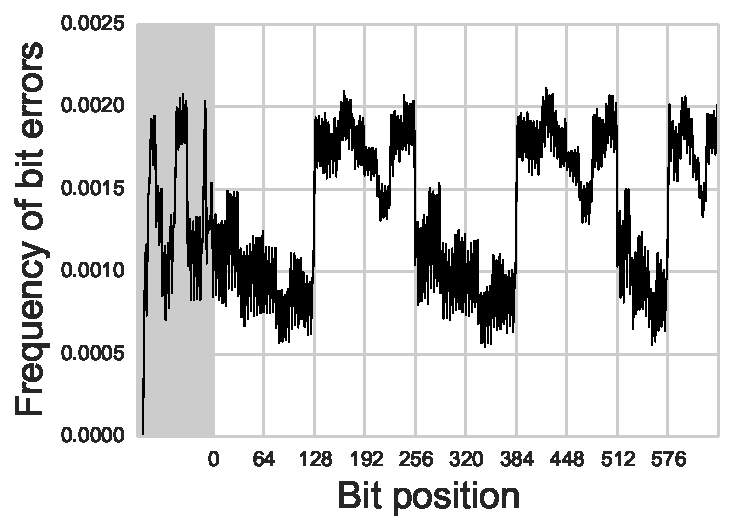
\includegraphics[width=0.475\columnwidth]{figures/8mote_0-5_xor_simulation}
		\label{fig:8mote_xl_xor_simulation}
	}
	\subfigure[Simulated S bit error pattern.] {
		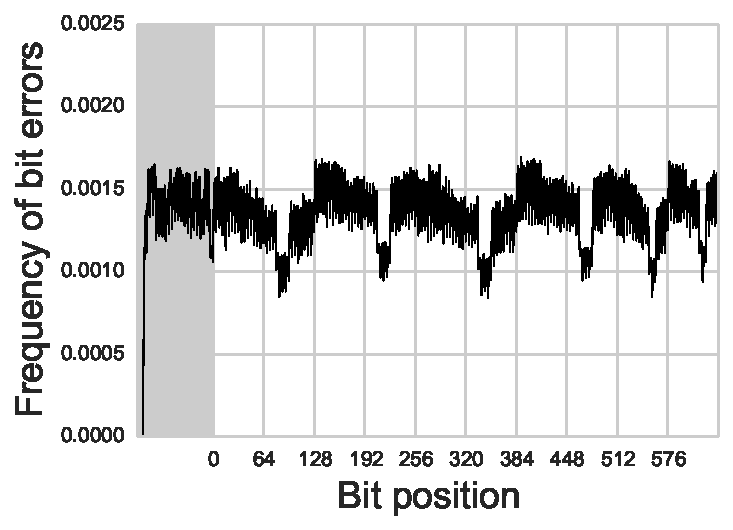
\includegraphics[width=0.475\columnwidth]{figures/8mote_2-7_xor_simulation}
		\label{fig:8mote_s_simulation}
	}
	\subfigure[Simulated XL burst error length.] {
		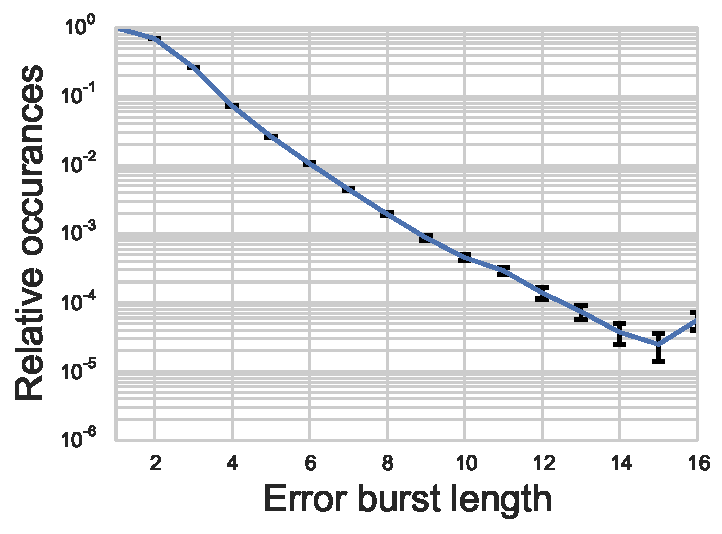
\includegraphics[width=0.475\columnwidth]{figures/8mote_0-5_burst_simulation}
		\label{fig:8mote_xl_burst_simulation}
	}
	\subfigure[Simulated S burst error length.] {
		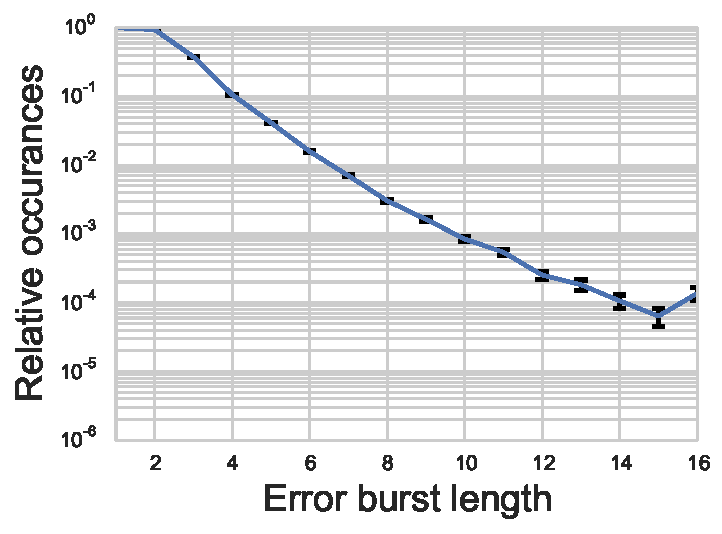
\includegraphics[width=0.475\columnwidth]{figures/8mote_2-7_burst_simulation}
		\label{fig:8mote_s_burst_simulation}
	}
	\caption{Error patterns of simulated constant payload using traces with constant payload. The error bars denote 99\% confidence intervals.}
	\label{fig:8mote_bit_errors_simulation}
\end{figure}

\paragraph{Packet Reception Rate}

To compare the overall number of corrupted messages of the original with the simulated link, we plotted the normalized \ac{PRR} of our original experiment with $RS(80,70)$ encoded payload and the simulation of that experiment with the same payload, as shown in Figures~\ref{fig:prr_link_01_fec} and \ref{fig:prr_link_10_fec} respectively.
To be able to compare the \ac{PRR} of encoded and non-encoded payload, we only evaluate the first $k=70$ bytes in the payload.
The timeouts shown in gray are the same for the simulation, since they are copied from the original, as mentioned before.

While the total amount of corrupted messages in the simulated link is the same as in the original link, as exemplified by the very similar error-free reception curves in the plots, error-free \ac{RS} decoded receptions yields slightly worse results, especially in areas with high byte error count, as visible in Figure~\ref{fig:prr_link_01_receiver_fec} and \ref{fig:prr_link_10_transmitter_fec}.
This shows that in these areas, the simulator overshoots the target bit error distribution of the original messages, and therefore undershoots the \ac{RS} decoded \ac{PRR} of the original link.
In the worst case, the simulated \ac{RS} performance is underestimated compared to reality, which is sufficient for our assessments.

\begin{figure}[t]
	\subfigure[Comparison of link~\ref{fig:prr_link_01_transmitter}.] {
		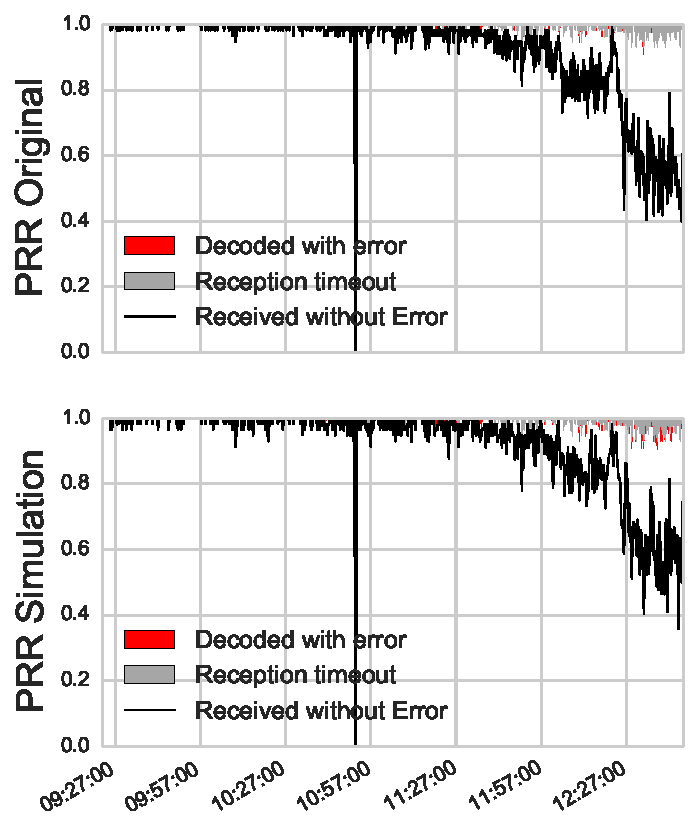
\includegraphics[width=0.475\columnwidth]{figures/fec_scheme_box0_box1_os_0-1_Throughput}
		\label{fig:prr_link_01_transmitter_fec}
	}
	\subfigure[Comparison of link~\ref{fig:prr_link_01_receiver}.] {
		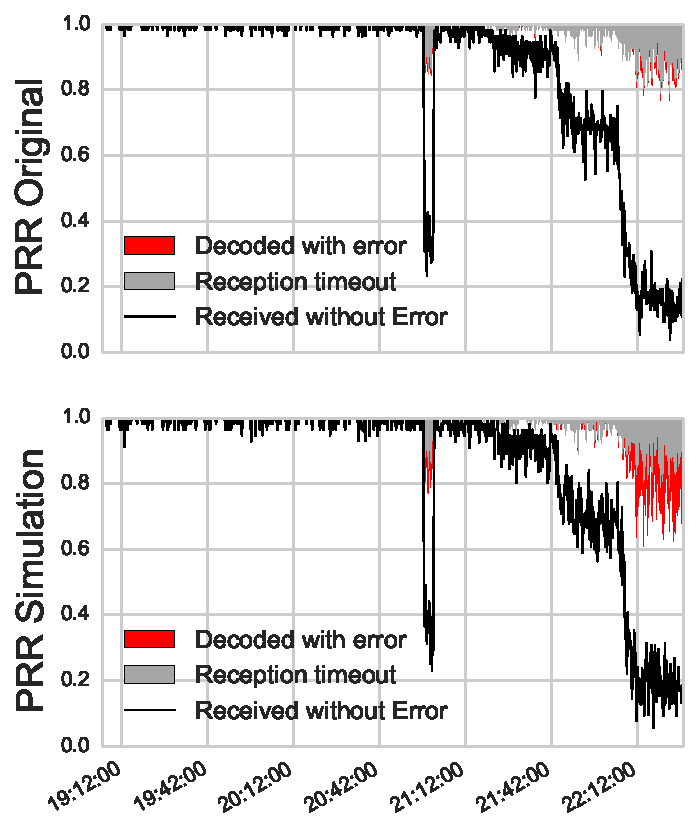
\includegraphics[width=0.475\columnwidth]{figures/fec_scheme_box1_box0_os_0-1_Throughput}
		\label{fig:prr_link_01_receiver_fec}
	}
	\caption{Original and simulated \acs{PRR} of the two $RS(80,70)$ encoded links of Figure~\ref{fig:prr_link_01}. Note the drop in simulated \acs{RS} decoded \acs{PRR} in (b).}
	\label{fig:prr_link_01_fec}
\end{figure}

\begin{figure}[t]
	\subfigure[Comparison of link~\ref{fig:prr_link_10_receiver}.] {
		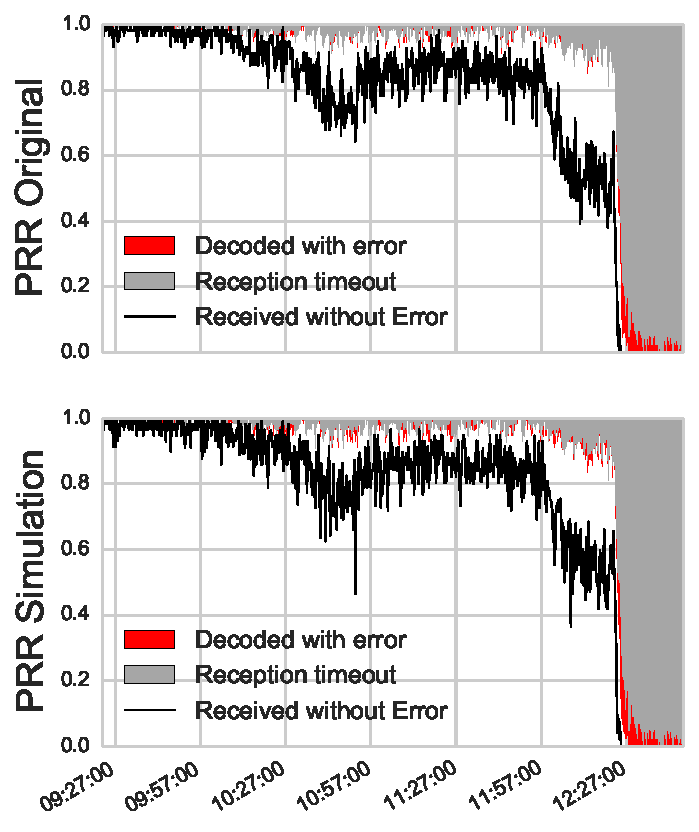
\includegraphics[width=0.475\columnwidth]{figures/fec_scheme_box0_box1_os_1-0_Throughput}
		\label{fig:prr_link_10_receiver_fec}
	}
	\subfigure[Comparison of link~\ref{fig:prr_link_10_transmitter}.] {
		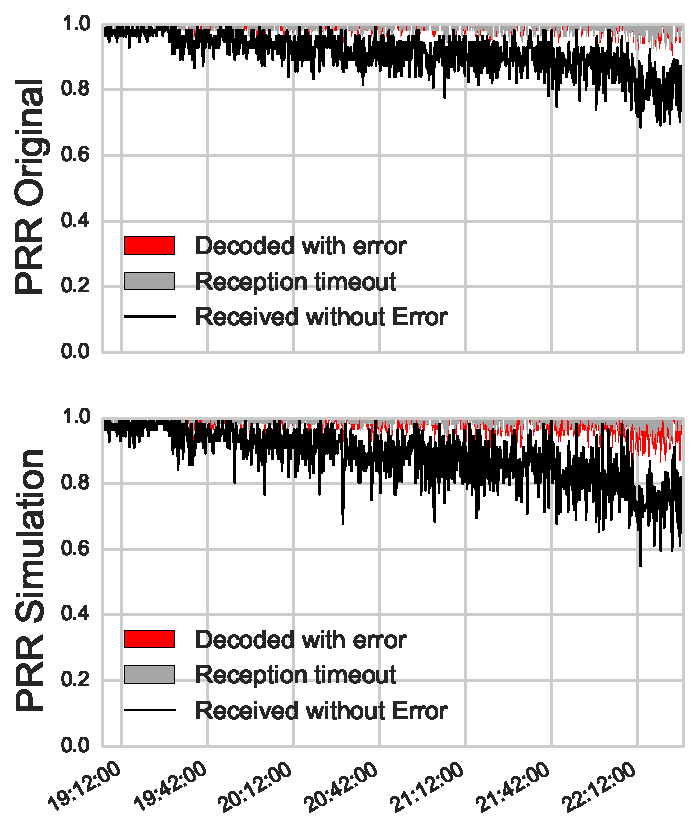
\includegraphics[width=0.475\columnwidth]{figures/fec_scheme_box1_box0_os_1-0_Throughput}
		\label{fig:prr_link_10_transmitter_fec}
	}
	\caption{Original and simulated \acs{PRR} of the two $RS(80,70)$ encoded links of Figure~\ref{fig:prr_link_10}.}
	\label{fig:prr_link_10_fec}
\end{figure}

These results show that this simple simulator is a very good time- and cost-saving alternative to testing the effects of different payloads over a real link, if good original data is available.
Using our trace-based simulator eliminates the effect of uncontrollable environmental factors or hardware issues on repeatability and allows us to focus purely on the message content, without assuming  idealized and monolithic link properties.


\section{Comparing \acs{RS} Scheme Strengths}

Our first idea was to keep a constant data size of $k=80$ and add parity bytes, making the entire message longer.
However, longer packets require more energy to transmit, a metric which has to be included somehow when comparing different $k$.
Furthermore, because of the size limit of the \ac{MPDU} of 127 bytes, of which 26 are already used, this only leaves $n=101$ bytes with a maximum of $n-k=19$ parity bytes, which would not allow to encode with more than 18\% coding overhead.
We could have split the message into two packets, however, this would have made it even harder to compare them, since now two packets must be received in the right sequence.

Therefore, we abandoned this idea and fit the entire encoded message into 80 bytes, including parity bytes as shown in Figure~\ref{fig:rs_codeword}.
This means we can only transfer $k$ bytes of encoded data, effectively reducing data rate while gaining robustness, which we want to use for a metric for comparing \ac{RS} performance.
We combine this reduction of data rate and the corruption of decoded packets as throughput, normalized over the number of \emph{received} messages.
We calculated the normalized throughput $T(80, k)$ using the following formula:

\[ T(80, k) = \frac{k}{80} \frac{PRR_{decoded}}{PRR_{received}} \]

This metric allows us to compare \ac{RS} performance not only between different coding strengths, but augment that comparison with context of the link's quality.
% The normalized throughputs of the original versus simulated links are also available in Figures~\ref{fig:prr_link_01_fec} and \ref{fig:prr_link_10_fec}.
% Especially the drop in Figure~\ref{fig:prr_link_01_receiver} visualizes the previous findings that the simulation slightly underestimates, but never overestimates \ac{RS} decoded \ac{PRR}.

For each of the four links discussed in Section~\ref{sec:packet_reception_rate} we simulated new $RS(80, k)$ encoded payload for $k$ in 10 byte increments up to $k=60$, then in 2 byte increments up to $k=78$.
We plotted the normalized throughputs $T(80, k)$ in Figure~\ref{fig:throughput_link_fec}, with the dashed line showing throughput without RS encoding.
The graphs illustrate that even using only 2 parity bytes at $k=78$ can already significantly improve \ac{PRR}, since most messages only have a few burst errors, and all those constrained to one byte can be corrected.

Adding two more parity bytes for $k=76$ improves \ac{PRR} even more, but only in a few areas.
From $k=74$ to $k=60$ no significant improvement shows, especially at low temperatures.
Using $k=60$ shows stability up to high temperature of $80\,^{\circ}\mathrm{C}$ in all Figures except \ref{fig:throughput_link_10_receiver_fec}.
At and below $k=50$ no improvement of throughput is visible except in Figure~\ref{fig:throughput_link_10_receiver_fec}, where $k=30$ and $k=20$ hold throughput the longest.

By comparing Figure~\ref{fig:prr_link_01_receiver_fec} and \ref{fig:throughput_link_01_receiver_fec}, we can deduct that in that link the simulated throughput above \SI{70}{\celsius} is actually worse than in reality. Therefore we can safely assume $k=60$ as stable at that temperature.

\begin{figure}[t]
	\subfigure[Simulated link~\ref{fig:prr_link_01_transmitter}.] {
		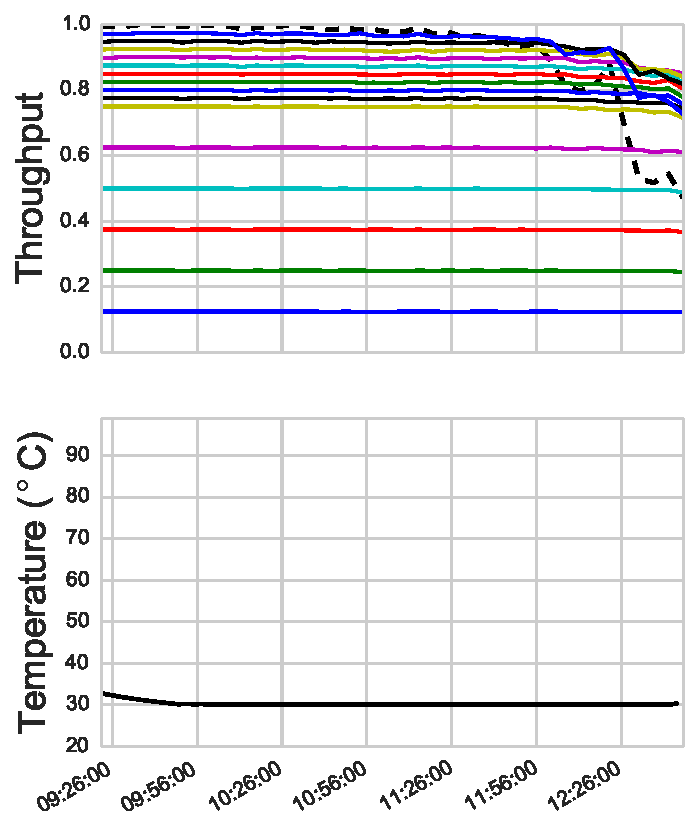
\includegraphics[width=0.475\columnwidth]{figures/fec_scheme_box0_box1_0-1_Throughput}
		\label{fig:throughput_link_01_transmitter_fec}
	}
	\subfigure[Simulated link~\ref{fig:prr_link_01_receiver}.] {
		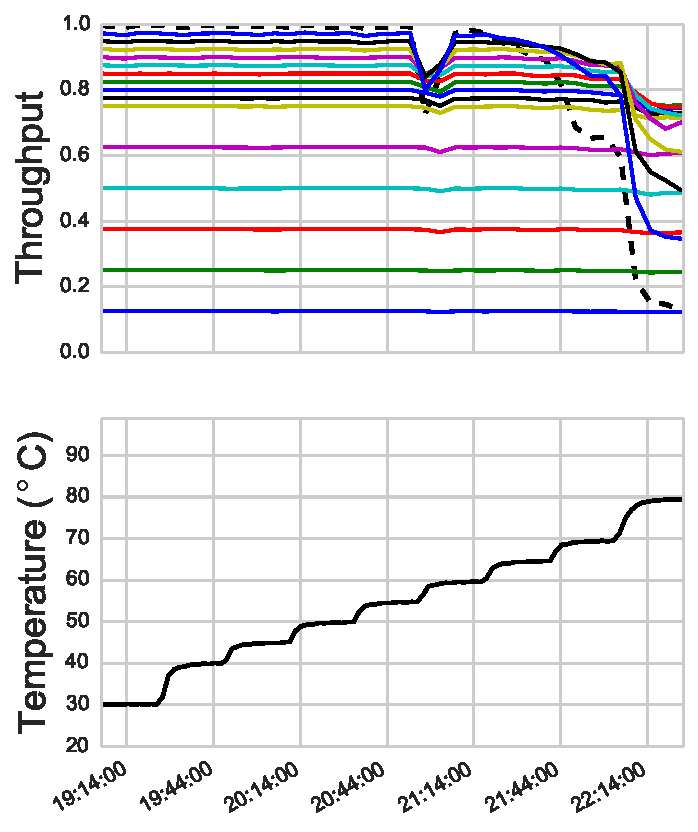
\includegraphics[width=0.475\columnwidth]{figures/fec_scheme_box1_box0_0-1_Throughput}
		\label{fig:throughput_link_01_receiver_fec}
	}
	\subfigure[Simulated link~\ref{fig:prr_link_10_receiver}.] {
		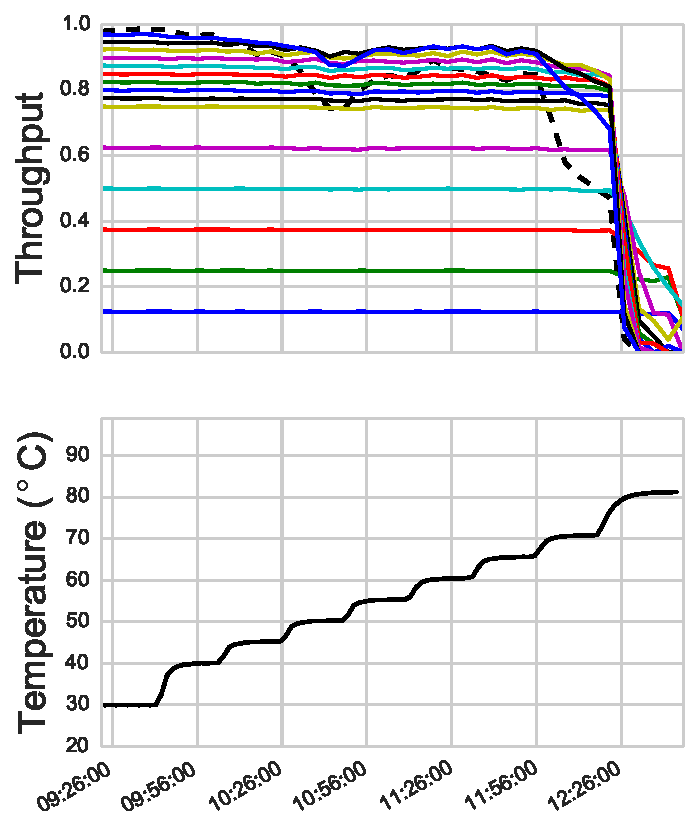
\includegraphics[width=0.475\columnwidth]{figures/fec_scheme_box0_box1_1-0_Throughput}
		\label{fig:throughput_link_10_receiver_fec}
	}
	\subfigure[Simulated link~\ref{fig:prr_link_10_transmitter}.] {
		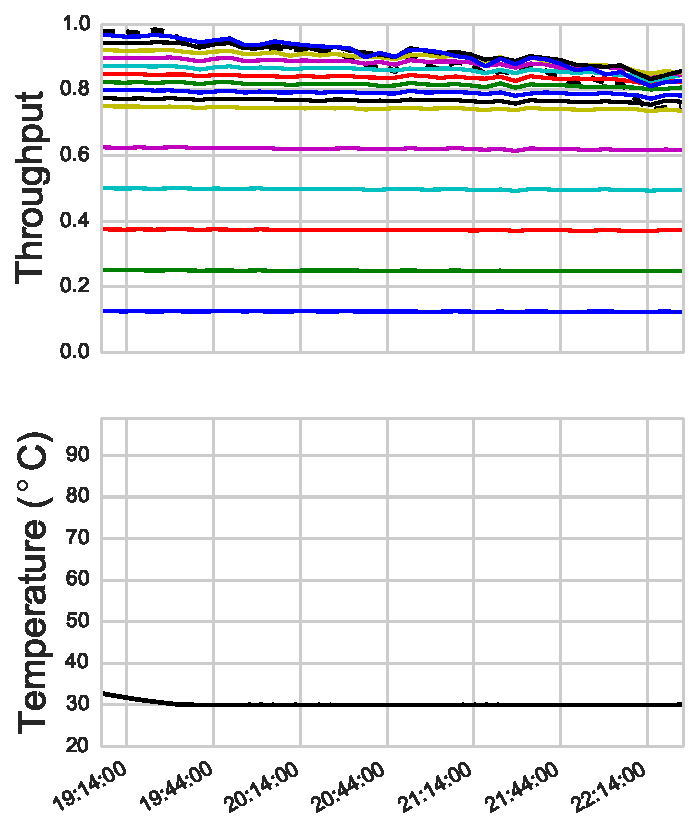
\includegraphics[width=0.475\columnwidth]{figures/fec_scheme_box1_box0_1-0_Throughput}
		\label{fig:throughput_link_10_transmitter_fec}
	}
	\caption{Comparison of throughputs $T(80, k)$ of all four simulated links of Section~\ref{sec:packet_reception_rate} for \\$k \in \{10,20,30,40,50,60,62,64,66,68,70,72,74,76,78\}$ over temperature. The dashed line shows throughput at $k=80$, which is equivalent to using no parity bytes.}
	\label{fig:throughput_link_fec}
\end{figure}



\section{Discussion}

Considering that the goal of using an \ac{FEC} in the context of low power networks such as \ac{WSN}s is to maximize energy efficiency of communications, we are not only looking for the $k$ with maximum throughput, but also with the least retransmissions.
We also have to consider that the link quality can already be poor at low temperature, therefore using no parity bytes at low temperatures is not a good idea either.

As per our findings, we propose one possible \ac{RS} scheme starting with $k=70$, which is 12.5\% overhead (the same as the popular $RS(255,223)$~\cite{Ma2009}), at low temperatures and linearly increase this to $k=60$ (or 25\% overhead) as receiver temperature increases to $70\,^{\circ}\mathrm{C}$ and above.
Starting with $k=70$ will give some protection against a random decrease in link quality as seen in Figure~\ref{fig:throughput_link_01_receiver_fec}.
In cases of extremely high bit error, such as in Figure~\ref{fig:throughput_link_10_receiver_fec}, we can still regain some throughput by using $60-80\%$ coding overhead with $k=30$ or $k=20$.
However, considering the extremely low \ac{PRR} in this area (compare with Figure~\ref{fig:prr_link_10_receiver_fec}), most of these messages will likely never be received anyway, which makes this option only viable when communication at these temperatures is absolutely necessary.

The results of Boano~\etal~\cite{Boano2013} strongly suggested that the loss in \ac{PRR} is more pronounced when heating the transmitter than the receiver.
This would have allowed us to use local temperature measurements to adapt the coding strength of our \ac{FEC} scheme to counteract the loss in \ac{PRR}.
Unfortunately, our results firmly oppose the findings of Boano~\etal{}: heating the receiver creates a higher loss in \ac{PRR} than heating the transmitter, therefore making such an approach unusable.
However, using temperature as another source for assessing link quality has the distinct advantage of being always available on the receiver locally, compared to \ac{LQI} and \ac{RSSI}, which requires a message to be received first.

We therefore propose another solution to adapt \ac{FEC} strength:
the receiver should monitor its local temperature and send out a warning broadcast to all potential transmitters, before its temperature becomes too high.
The transmitters can then address this mote with the appropriate \ac{FEC} strength.
The advantage of this active, preemptive approach over backchanneling link quality information is that in setups where transmissions only occur sparsely, a ``test'' transmission to judge link quality is not required.




\chapter{Conclusion}

This work investigated the effects of temperature on bit error patterns and \ac{PRR} in the context of low power communications as used in \acp{WSN}.

We began with a description of the low-cost design of our testbed, which allows fine control of mote temperature, mote orientation and experiment execution.
This testbed was the foundation, which allowed us to create and control links with high \ac{BER} between CC2420 radios at different temperatures.
Due to problems with the serial communication between mote and PC, we measured microcontroller clock drift and found the \ac{DCO} calibration algorithm in TinyOS not to be working above \SI{55}{\celsius}, and provided and tested a correction method.

Then we showed that bit errors follow a distinct distribution, which is influenced by payload content, confirming findings by Schmidt~\etal~\cite{Schmidt2013} and extending them with a classification of pattern magnitudes.
We found two bit error patterns, which we did not know before, due to their rare occurrence.
Furthermore, we saw no influence of temperature on these patterns.

The experiments were completed with a detailed investigation into \ac{PRR} asymmetry, when transmitter and receiver were heated to different temperatures.
Our results showed that the receiver is more vulnerable to an increase in temperature than the transmitter, thereby disproving findings by Boano~\etal~\cite{Boano2013}.

We used these findings to create a trace-based simulator to study the effects of temperature on \ac{FEC} usage, and evaluated the simulators performance, which we found accurate.
Using traces of our real experiments, we simulated several \ac{RS} encoding strengths and compared them based on normalized throughput.
On this basis we proposed a minimum encoding strength of 12.5\% overhead, which is increased with temperature to a maximum of 25\% overhead.



% It seems we are missing a independent \ac{LQE} across platforms and testbeds.
% This exact problem has been summarized by Baccour~\etal{} in their survey~\cite{Baccour2012}.
% The authors come to the conclusions that of the hardware-based \ac{LQE}s, \ac{RSSI} has the worst accuracy, especially for intermediate links, and that \ac{LQI} is a better indicator of \ac{PRR} than \ac{RSSI}, as we have pointed out too.
% They come to the conclusion that software-based \ac{LQE}s are better at describing link quality than hardware-based \ac{LQE}s.

\newpage

\section*{Future Work}

The results of our experiment warrant further investigations into several topics.

In Section~\ref{sec:link_quality} we briefly described the difficulty we encountered in creating a link with the right \ac{BER} even when using our mote harness from Section~\ref{sec:mote_harness}.
An interesting addition to this harness could be a motor controlled z-axis to further automate link quality selection via antenna orientation in a closed-loop controller setup.
In that respect, it might be more practical to rebuild this harness partially out of LEGO Technic parts, which would make the mechanic aspects of this function much easier.

Concerning the limitations of the \ac{DCO} calibration algorithm of TinyOS described in Section~\ref{sec:clock_drift}, we filed a bug report on their open-source project page.
We hope that this raises awareness of the algorithm's performance and prompts a fix.

In Section~\ref{subsec:pattern_anomalies} we described two bit error patterns, which were very different to what we recorded in all other experiments we ran.
Further investigation is required to understand what creates these patterns and whether they exhibit different Hamming distances than described by Schmidt~\etal~\cite{Schmidt2013} and Hermans~\etal~\cite{Hermans2014}.

Further work is required to validate our proposals regarding temperature dependent \ac{RS} coding overhead using simulation and real experiments.
Even though our simulation was accurate enough for our conclusions, they were based on four real traces, which certainly do not cover all possible link qualities that can be expected in real world deployments.

% It is important to notice, that in regions with high link quality, especially at low temperature, \ac{ARQ} might outperform \ac{FEC} in energy efficiency as reported by Tian~\etal~\cite{Tian2008}.
% Therefore our results might be best deployed in a hybrid \ac{ARQ} scheme~\cite{Liu1997}, where \ac{FEC} is only deployed once the temperature reaches a certain threshold.


% \todo{we logged all raw data, so we could use it to test software-based \ac{LQE}s~\cite{Baccour2012}}

% \todo{Correlation threshold of the CC2420 can be user defined~\cite{Liang2010}}

% This link asymmetry can lead to some interesting situations, where a mote at high temperature is able to transmit messages, but not receive them.
% Looking at their own temperature, mote would receive another hint in whether the lack of received messages is caused by a missing transmitter, or by its own disability to receive messages.
% For example, when no messages are received after a timeout, a failure of the transmitter is more likely when the receiver is at low temperature than at high temperatures.

% In a system that makes smart decisions based on information from multiple motes, such information could be used to judge whether the system is still functionally intact and then trigger a backup program, which reacts autonomously to the local sensor data collected but still notifies the rest of the network of its actions.
% Motes that are not in this backup mode can very likely receive these transmissions and augment the group decisions with the constraints of these autonomously acting motes.
% Therefore a failure of the entire system is delayed or prevented, by using controlled degradation of the system, which might not be as smart as before, but at least still providing a rudimentary service.


%%%%%%%%%%%%%%%%%%%%%%%%%%%%%%%%%%%%%%%%%%%%%%%%%%%%%%%%%%%%%
%% LITERATUR UND ANDERE VERZEICHNISSE
%%%%%%%%%%%%%%%%%%%%%%%%%%%%%%%%%%%%%%%%%%%%%%%%%%%%%%%%%%%%%
%% Ein kleiner Abstand zu den Kapiteln im Inhaltsverzeichnis (toc)
\ifnotdraft{
\addtocontents{toc}{\protect\vspace*{\baselineskip}}
\cleardoublepage
%% Literaturverzeichnis
\phantomsection % phantomsection wird benötigt, damit z.B. hyperref die richtige Seite verlinkt.
\addcontentsline{toc}{chapter}{Bibliography}
%\nocite{*} %Auch nicht-zitierte BibTeX-Einträge werden angezeigt.
\bibliography{literature/literature}%Eine Datei 'literatur.bib' wird hierfür benötigt.
\bibliographystyle{acmurl}%Art der Ausgabe: plain / apalike / amsalpha / ...
}

%% Abbildungsverzeichnisgitx

%\clearpage
%\addcontentsline{toc}{chapter}{List of Figures}
%\listoffigures

%% Tabellenverzeichnis
%\clearpage
%\addcontentsline{toc}{chapter}{List of Tables}
%\listoftables


%%%%%%%%%%%%%%%%%%%%%%%%%%%%%%%%%%%%%%%%%%%%%%%%%%%%%%%%%%%%%
%% ANHÄNGE
%%%%%%%%%%%%%%%%%%%%%%%%%%%%%%%%%%%%%%%%%%%%%%%%%%%%%%%%%%%%%
\appendix
\chapter{Appendix}

\section{List of Abbreviations}

\begin{acronym}[MOSFET]
	\setlength{\itemsep}{-\parsep}
	
	\acro{MOSFET}{Metal–Oxide–Semiconductor Field-Effect Transistor}
	\acro{ISP}{In-System Programming}
	\acro{PRR}{Packet Reception Rate}
	\acro{PID}{Proportional-Integral-Derivative}
	\acro{ATX}{Advanced Technology eXtended}
	\acro{DCO}{Digitally Controlled Oscillator}
	\acro{UART}{Universal Asynchronous Receiver Transmitter}
	\acro{BER}{Bit Error Rate}
	\acro{LQI}{Link Quality Indication}
	\acro{RSSI}{Received Signal Strength Indication}
\end{acronym}


\begin{table}
	\subtable[Average Packet Reception Rate in \%]
	{
		\begin{tabularx}{\linewidth}{|c*{4}{|d{-1}}|}
		\hline
		\T \cellcolor{slightgray} Receiver	& \multicolumn{1}{X|}{\cellcolor{motered} \centering Sender 0} & \multicolumn{1}{X|}{\cellcolor{motered} \centering Sender 1} & \multicolumn{1}{X|}{\cellcolor{moteblue} \centering Sender 2}	& \multicolumn{1}{X|}{\cellcolor{moteblue} \centering Sender 3}\\
		\hline

		\cellcolor{moteblue}\T 4 & \cellcolor{slightred} 3.2  & \cellcolor{slightgreen} 96.9 & \cellcolor{slightred} 5.5  & \cellcolor{slightgreen} 100.0 \B\\
		\hline
		\cellcolor{motered}\T 5 & 81.9 & 87.2 & \cellcolor{slightred} 0.4  & \cellcolor{slightgreen} 99.2 \B\\
		\hline
		\cellcolor{moteblue}\T 6 & \cellcolor{slightgreen} 98.1 & 75.2 & 89.9 & \cellcolor{slightred} 0.1  \B\\
		\hline
		\cellcolor{motered}\T 7 & \cellcolor{slightgreen} 96.2 & \cellcolor{slightred} 2.0    & 57.3 & 44.0	\B\\
		\hline 
		\end{tabularx}
	}

	\subtable[Average Error Free Packets Reception Rate in \%]
	{
		\begin{tabularx}{\linewidth}{|c*{4}{|d{-1}}|}
		\hline
		\T \cellcolor{slightgray} Receiver	& \multicolumn{1}{X|}{\cellcolor{motered} \centering Sender 0} & \multicolumn{1}{X|}{\cellcolor{motered} \centering Sender 1} & \multicolumn{1}{X|}{\cellcolor{moteblue} \centering Sender 2}	& \multicolumn{1}{X|}{\cellcolor{moteblue} \centering Sender 3}\\
		\hline

		\cellcolor{moteblue}\T 4 & \cellcolor{slightred} 0.0  & 69.5 & \cellcolor{slightred} 2.7  & \cellcolor{slightgreen} 100.0 \B\\
		\hline
		\cellcolor{motered}\T 5 & \cellcolor{slightred} 7.1 & 10.8 & \cellcolor{slightred} 0.0  & 88.3 \B\\
		\hline
		\cellcolor{moteblue}\T 6 & 83.8 & \cellcolor{slightred} 2.1 & 22.1 & \cellcolor{slightred} 0.0  \B\\
		\hline
		\cellcolor{motered}\T 7 & \cellcolor{slightgreen} 96.0 & \cellcolor{slightred} 0.1    & \cellcolor{slightred} 9.8 & \cellcolor{slightred} 1.4	\B\\
		\hline 
		\end{tabularx}
	}

	\subtable[Average LQI values]
	{
		\begin{tabularx}{\linewidth}{|c*{4}{|d{-1}}|}
		\hline
		\T \cellcolor{slightgray} Receiver	& \multicolumn{1}{X|}{\cellcolor{motered} \centering Sender 0} & \multicolumn{1}{X|}{\cellcolor{motered} \centering Sender 1} & \multicolumn{1}{X|}{\cellcolor{moteblue} \centering Sender 2}	& \multicolumn{1}{X|}{\cellcolor{moteblue} \centering Sender 3}\\
		\hline

		\cellcolor{moteblue}\T 4 & \cellcolor{slightred} 50 & 79 & \cellcolor{slightred} 77 & \cellcolor{slightgreen} 101 \B\\
		\hline
		\cellcolor{motered}\T 5 & 71 & 72 & \cellcolor{slightred} 49  & 87 \B\\
		\hline
		\cellcolor{moteblue}\T 6 & 85 & 67 & 73 & \cellcolor{slightred} 35  \B\\
		\hline
		\cellcolor{motered}\T 7 & \cellcolor{slightgreen} 106 & \cellcolor{slightred} \cellcolor{slightred} 44 & 65 & 61	\B\\
		\hline 
		\end{tabularx}
	}

	\caption{Complete table of link qualifiers from the experiment described in Subsection~\ref{subsec:effects_of_board_layout}. Good links (PRR > 90\%) are marked green, bad links (PRR < 10\%) red. Notice the distinction between PRR in Table (a) and \emph{error-free} PRR in Table (b) in comparison to LQI in Table (c).}

	\label{tab:8mote_link_qualities}
\end{table}

\end{document}
